\documentclass[conference]{IEEEtran}
\IEEEoverridecommandlockouts
% The preceding line is only needed to identify funding in the first footnote. If that is unneeded, please comment it out.
\usepackage{cite}
\usepackage{amsmath,amssymb,amsfonts,amsthm}
\usepackage{graphicx}
\usepackage{textcomp}
\usepackage{xcolor}
\usepackage[noend]{algpseudocode}
\usepackage{algorithmicx,algorithm}
% \usepackage{caption}
\usepackage{forest}
\ifCLASSOPTIONcompsoc
\usepackage[caption=false,font=normalsize,labelfont=sf,textfont=sf,position=top]{subfig}
\else
\usepackage[caption=false,font=footnotesize]{subfig}\fi

\def\BibTeX{{\rm B\kern-.05em{\sc i\kern-.025em b}\kern-.08em
    T\kern-.1667em\lower.7ex\hbox{E}\kern-.125emX}}
\begin{document}

% \theoremstyle{definition}
\newtheorem{definition}{Definition}
\theoremstyle{definition}
\newtheorem{example}{Example}
\theoremstyle{plain}
\newtheorem{theorem}{Theorem}

\newtheorem{lemma}{Lemma}


\title{Frequent Itemset Mining Under Differential Privacy with Multiple Minimum Supports}

\author{\IEEEauthorblockN{1\textsuperscript{st} Yum-Luh Wang}
\IEEEauthorblockA{\textit{Graduate Institute of Electronics Engineering} \\
\textit{National Taiwan University}\\
Taipei, Taiwan \\
r07943161@ntu.edu.tw}
\and
\IEEEauthorblockN{2\textsuperscript{nd} Yao-Tung Tsou}
\IEEEauthorblockA{\textit{Department of Communications Engineering} \\
\textit{Feng Chia University}\\
Taichung, Taiwan \\
yttsou@fcu.edu.tw}
\and
\IEEEauthorblockN{3\textsuperscript{rd} Sy-Yen Kuo}
\IEEEauthorblockA{\textit{Graduate Institute of Electronics Engineering} \\
\textit{National Taiwan University}\\
Taipei, Taiwan \\
sykuo@ntu.edu.tw}
}

\maketitle

\begin{abstract}%可以
Frequent itemset mining is an extensively studied research domain of data mining. The aim is to find interesting correlations between items in a transaction database. 
However, malicious user might gain sensitive information in the mining process. 
Differential privacy is the de facto standard when it comes to protecting data. 
Combining differential privacy with frequent itemset mining can provide strong privacy guarantee while generating statistical information from sensitive data.
In existing studies, most algorithms are focusing on finding frequent patterns using one predefined threshold with the protect of differential privacy.
However, using single threshold to extract itemsets creates ``rare item problem'', and setting respective support thresholds for each item is more adequate to reflect the nature of widely varied items.
In this paper, we propose a novel FP-growth-like solution DPCFP++ to solve the rare item problem of frequent itemset mining while guarantee differential privacy at the same time.
The experiments illustrate that our algorithm acheieves high utility in privately solving rare item problem.
\end{abstract}

\begin{IEEEkeywords}
Differential Privacy, data mining, multiple minimum supports, frequent itemset mining
\end{IEEEkeywords}

\section{Introduction}%最後一段還沒
In modern era, the development of information technology grows rapidly, more and more services aggregate data from individuals. 
With the evolution of machine learning and statistics, organizations utilize these enormous amount of data to improve the accuracy of their model, understand the past and predict the future.
Frequent itemset mining is a popular research topic in data mining, and it was first introduced in 1993 by Agrawal et al.\cite{b1} 
The original purpose of frequent itemset mining was to analyze customer habits in a supermarket. 
They tried to find associations between different items that customers frequently bought together. 
According to the mined results, the management team of the supermarket can make business decisions to maximize profit including product rearrangement, bundle selling, etc.
After decades of research, frequent itemset mining can also be extended to many other area besides market basket analysis. For example, text mining, disease diagnosis, and so on.

Majority of existing literatures endeavors on single threshold mining, that is, treat all the items equally and apply a single threshold to decide whether an itemset is frequent or not.
However, setting one appropriate threshold for all items is a hard question. 
For example, consider two items: soda and television in a wholesale store. Soda is frequently bought while television is an uncommon purchase. 
If the threshold is set too high, we might consider TV as a less important item, but TV contributes thousand times more to the store revenue than the common purchased soda. 
On the other hand, if the threshold is too low, the computational cost becomes expensive, the mining result will cause combinational explosion and we will receive many meaningless itemsets. 
The above dilemma is the famous ``rare item problem''. In real life applications, some items tend to have more weights in natural than other items. 
Researchers \cite{b2}\cite{b3}\cite{b4}\cite{b5} have worked on this problem by allowing users to use ``multiple minimum supports''. 
Briefly speaking, rare itemset mining is a more advanced setting of frequent itemset mining, and it allows user to apply different threshold on each item .

The convenience which data mining brings comes with the price of privacy leakage. The more precise the model is, the more personal behavioral information reveals. 
How to de-identification is a mainstream topic in related research.
A straightforward approach is to .......

Differential Privacy, first proposed by Dwork in\cite{b4}, had come to rescue in 2006. 
Since then, many research based on differential privacy have been conducted. Tech giants such as FAANG(facebook, applem, amazon, netflix, google) have added features to their products with different kinds of differential privacy model.
% Differential privacy is the {\it{de facto}} standard for protecting privacy. 
It guarantees that the outputs of a mechanism will be approximately the same when two input is almost identical, and thus protect privacy from explosure. 

It guarantees that a user.........
In this paper, we study the problem of how to perform frequent itemset mining (FIM) on transaction databases while satisfying differential privacy.


\section{Related Work}
\subsection{Frequent Itemset Mining}
There are mainly two types of frequent itemset mining algorithms. 
One is Apriori, and the other is FP-growth. %%APriori and FP!!
\subsection{Frequent Itemset Mining with Multiple Minimum Supports}

\subsection{Differentially Private Frequent Itemset Mining}

Frequent itemset mining, also known as frequent pattern mining, is 
The NoisyCut algorithm in \cite{b8} was proven violating differential privacy in %%cite!


%第三段囉
\section{Preliminaries and Problem Statement}
In this section, we introduce and provide formal definitions of differential privacy and the rare item problem of frequent itemset mining. 
Finally, we give the problem statement in the last subsection.

\subsection{Differential Privacy}%definition 
Differential privacy guarantees that the presence or absence of any individual will not significantly change the output of an algorithm.
By this approach, one can only infer limited information about that particular individual from the output.

\begin{definition}{($\varepsilon$-Differential Privacy):}\\
Let $D$ and $D'$ denote two neighboring databases, which means they differ by at most one record.
A mechanism $\mathcal{M}$ is $\varepsilon$-differential private if and only if for any $S \subseteq Range(\mathcal{M})$
\begin{equation}
Pr[\mathcal{M(D)}\in S] \leq e^\varepsilon \cdot Pr[\mathcal{M(D')}\in S]
\end{equation}
\end{definition}
The parameter $\varepsilon$ is called privacy budget, it quantifies the degree of privacy.
The larger the $\varepsilon$, the less private the result is. If the $\varepsilon$=0, the result is perfectly private. 

There are a few mechanisms that acheieves differential privacy.
Laplace mechanism is one of the most popular method. 
It injects properly calibrated noise into the original output according to the sensitivity.
We give the definition of sensitivity as follows.

\begin{definition}{(Sensitivity):}\\
When answering numeric queries of neighboring databases, the sensitivity of a query Q is 
\begin{equation}
\bigtriangleup_Q=\mathop{max}\limits_{D,D'}\Arrowvert Q(D)-Q(D') \Arrowvert_1
\end{equation}
\end{definition}
Sensitivity is used to measure the maximum possible change in the outputs over any two neighboring databases.

\begin{definition}{(Laplace Mechanism):}\\
For any function $Q:D\rightarrow R$, Laplace mechanism $\mathcal{M}$ satisfies $\varepsilon$-differential privacy by adding noise to the origin output:
\begin{equation}
    \mathcal{M}(D) = Q(D)+Lap(\frac{\bigtriangleup_Q}{\varepsilon}),
\end{equation}
where $Lap(\frac{\bigtriangleup_Q}{\varepsilon})$ is the noise drawn i.i.d from the Laplace distribution with scale $\frac{\bigtriangleup_Q}{\varepsilon}$.
\end{definition}
% seqential post-processing
There are some qualitative properties of differential privacy. We will use following properties in our solution. 

\begin{lemma}{(Sequential Composition):}\\\label{lm1}
Given an algorithm $\mathcal{M}$ consisting of a sequence of procedures $\{\mathcal{M}_1,\mathcal{M}_2,\dots,\mathcal{M}_n\}$. 
If each procedure $\mathcal{M}_i$ satisfies $\varepsilon_i$-differential privacy, then $\mathcal{M}$ satisfies $\sum_{i=1}^n\varepsilon_i$-differential privacy.
\end{lemma}

\begin{lemma}{(Closure Under Post-Processing):}\\\label{lm2}
    For any algorithm $\mathcal{A}$ and a $\varepsilon$-differentially private mechanism $\mathcal{M}$,
    the computaion $\mathcal{A}\circ\mathcal{M}(D)$ satisfies $\varepsilon$-differential privacy as long as $A$ do not access database directly.
    
\end{lemma}


\subsection{Frequent Itemset Mining}
Given a threshold  $\lambda$ and a transaction database $D=\{t_1,t_2,t_3,\dots,t_n\}$ consisting of $n$ transactions where each transaction is composed of sets of distinct items in the item universe $I=\{i_1,i_2,i_3,\dots,i_m\}$, i.e. $t_j\subseteq I$,
Frequent itemset mining, also known as frequent pattern mining, refers to discovering all set of patterns while the support of which is greater than or equal to a user-specified threshold.

\begin{definition}{(Itemset):}\\
Any subset of the item universe I is called an itemset.
\end{definition}
An itemset which contains k distinct items is called k-itemset. k is also called the length of the itemset or the cardinality of the itemset. 
We will use them in this work interchangebly.


\begin{definition}{(Support and Threshold):}\\
The number of transactions in the database containing an itemset is known as the support of that itemset.
\end{definition}
We denote support and threshold as $S$ and $\lambda$, respectively.
There are two ways to specify $\S$ and $\lambda$. One is the percentage way, and the other is by absolute number.
It is simple to convert between them, just multiply or divide the number of total transactions $n$.
% For consistency, we choose the former one in this paper.

\begin{definition}{(Frequent Itemset):}\\
An itemset $X$ is frequent if and only if its support $sup(X)$ is greater than or equal to support threshold $\lambda$.
\end{definition}
This means that the presence of itemset $X$ in the database is statistically significant.



\begin{table}[htbp]
    \caption{A Transaction Database}\label{db}
    \centering
    \begin{tabular}{|l|l|}
    \hline
    TID & \multicolumn{1}{c|}{Items} \\ \hline
    1   & a,b   \\ \hline
    2   & a,b,e \\ \hline
    3   & a,b,f \\ \hline
    4   & b,e,f \\ \hline
    5   & b,c   \\ \hline
    6   & a,b,e \\ \hline
    7   & b,c,g,h \\ \hline
    8   & e     \\ \hline
    9   & c,d   \\ \hline
    10  & c,d   \\ \hline
    \end{tabular}
    \begin{tabular}{|l|l|}
    \hline
    TID & \multicolumn{1}{c|}{Items} \\ \hline
    11  & a,e,d          \\ \hline
    12  & b,e        \\ \hline
    13  & a,b         \\ \hline
    14  & a,b,f        \\ \hline
    15  & b,f      \\ \hline
    16  & b,c,d,e,f,h  \\ \hline
    17  & a,e        \\ \hline
    18  & b,c,d          \\ \hline
    19  & a,e,g         \\ \hline
    20  & c,d        \\ \hline
    \end{tabular}
\end{table}

\begin{example}\label{ex1}
Consider the database shown in Table \ref{db}. There are $n=20$ transactions in the database, and item universe $I=\{a,b,c,d,e,f,g,h\}$.
The itemset (a,b) is a 2-itemset. It occurs in the database 6 times, so the $S$(a,b) is 6. 
Let's say the user-specified threshold is 2 and we can see (a,b) is a frequent itemset while (a,g) is not, for $S$(a,g) = 1.
\end{example}

\subsection{Rare Item Problem}
By the nature of items, some items appear more frequently than others. However, this sometimes causes meaningless itemsets.
We have to find frequent itemsets without generating too many meaningless itemsets.
To deal with rare item problem, Liu et al.\cite{b2} first tackled the problem with minimum item supports (MIS).
MIS allows user to specify respective threshold for every item. 
\begin{definition}{(Minimum Item Support)}\\
Minimum Item Support refers to each item's respective user-defined threshold.
\end{definition}
MIS can not only be set by user one by one, but also can be set adaptively.
Liu et al. also proposed a equation for fast-setting MIS by items' supports.
For an item $i_j$ with support $sup(j)$, the Minimum Item Support(MIS) of $j$ is
\begin{equation} 
MIS(i_j)=max\{\beta*sup(i_j),\lambda\},\label{eq}
\end{equation}
where $\beta\in[0,1]$.
$\beta$ is a relevance parameter that controls how the MIS values for items should be related to their frequencies.
Noted that when $\beta$=0, the MIS value equals $\lambda$, which is the same as the traditional setting of frequent itemset mining.


\begin{definition}{(MIS of an Itemset)}\\
The minimum item support of a k-itemset $X=\{i_1,i_2,i_3,\dots,i_k\}$ is the smallest MIS value of items in $X$, i.e. \\
\begin{equation} 
MIS(X)=min\{MIS(i_j)|i_j\in X\}.\label{eq2}
\end{equation}
\end{definition}

\begin{example}\label{ex2}
Consider the database in Table \ref{db}. 
If we set MIS(b)=15 and MIS(f)=3, then itemset (b) is not frequent since $S$(b) = 13. 
However, itemset (bf) is a frequent itemset since its support is 3 which is equal to MIS(bf) = min\{MIS(b),MIS(f)\} = 3.
\end{example}
Example \ref{ex2} shows that frequent itemset mining using multiple minimum supports is different from single threshold.
Under single threshold condition, if an itemset is not frequent, its superset is not frequent either.
This principle is called Apriori property, or downward closure property. 
However, Apriori property cannot be directly applied to our problem.


\subsection{Problem Statement}
Based on above definitions, we give the formal statement of our problem. 
Our algorithm works in a centralized model. As illustrate in Figure. %%figure
Given a transaction database, a threshold and a privacy budget, we want to find all frequent itemsets whose support is no less than the threshold using multiple minimum supports in a differentially private way.
\subsection{Main Challenges}
We oberserve there are two major challenges in using multiple minimum supports to mine frequent itemsets under differential privacy.
\begin{enumerate}
    \item {\it High Sensitivity}\\
    A straightforward approach is to count up each item's support, and direct apply Laplace noise to it. After that we can use traditional FIM algorithm to solve the problem.
    However, as we illustrate in the following example, this way is not practical.
    \begin{example}
        Consider a relatively tiny database which just contains 100 different items.
        If there is a transaction containing all 100 items, and its neighboring database doesn't, then when we start counting supports, all 100 items' support will change.
        Hence the sensitivity is 100 which is large, and we need to apply a tremendous amount of noise to achieve differential privacy. 
        As a consequence, the enormous noise we add would make the output of traditional FIM algorithm meaningless.
    \end{example}
    
    \item {\it Running Time}\\
    Most FIM algorithms under differential privacy is time-consuming. 
    We want to develope an algorithm that is agile and scans database as less as possible.
    An FP-growth-like algorithm doesn't generate candidate itemsets and it significantly scans database less than Apriori-like algorithm does.
    As a result, we aim to build an algorithm based on FP-growth.
    
\end{enumerate} 


\section{Proposed Method}
\subsection{Overview}
We now describe the framework of our proposed algorithm, which is called DPCFP, in the following paragraph. 
Motivated by the success in \cite{b4}\cite{b6}\cite{b8}, we combine their advantage together in this paper. 
DPCFP consists of three stages, namely {\it{TruncateDatabase}, \it{MISAssigning}, \it{CFP-Growth}.} 
The basic idea is to differential privately get each item's support and MIS. 
Next, we sort the items according to the descending order of MIS and put them into MIS header table. 
Afterwards, we add transactions into MIS-tree by the same order one after another. 
Finally, we use a FP-growth-like algorithm to find frequent itemsets.
Each step consumes different degrees of privacy budget, $\varepsilon_1$, $\varepsilon_2$,and $\varepsilon_3$, respectively.
$\varepsilon_1$, $\varepsilon_2$,and $\varepsilon_3$ follows the sequential composition rule of differential privacy, and hence the sum of them is the amount of privacy budget that user allocated.

\subsection{Truncate Database}
% Reference \cite{b6} is the first literature that tackle the high sensitivity problem by constrain the maximal number of items in transactions.
In this part, we truncate database to limit sensitivity to a acceptable level as \cite{b6} proposed.
The rationale behind truncating is that most transactions in a database is short in general case.
If there exist a few long transactions, then sensitivity will be affected remarkably.
These few long transactions which have major impact on sensitivity but less importance on frequent itemsets is infuriating.
To avoid this problem, we pose a limit to the length of transasctions. 
Of course, get rid of some items in transactions will create degrees of information loss.
\begin{algorithm}[htbp]
    \caption{TruncateDatabase} 
    \hspace*{0.02in} {\bf Input:} 
    database $D$; privacy budget $\varepsilon_1$;\\
    \hspace*{0.02in} {\bf Output:} %算法的结果输出
    truncated database $D'$
    
    \begin{algorithmic}[1]
    \State $D'\leftarrow \emptyset$
    \State Read $D$ to get total items $m$ and the total number of transactions $n$
    \State $z$ = {EstimateDistribution}{($D$, $\varepsilon_1$, $n$, $m$)}
    \State Let $l$ be the smallest integer such that  $\sum_{i=1}^l$$z_i$ $\ge$ 0.95
    \For{each transaction $t$ in $D$}
        \State add $t'$ = RandomTruncate($t$, $l$) to $D'$
    \EndFor 
    \State \Return $D'$
    
    \Function{EstimateDistribution}{$D$,$\varepsilon$,$n$,$m$} 
    \State Let $z = [ z_1, z_2, z_3,\dots,z_m]$, 
    where\ $z_i$\ is\ the\ number\ of\ transactions\ with\ cardinality\ $i$\ in $D$
    \State $z' = z + [Lap_1,Lap_2,Lap_3,...,Lap_m]$, where $Lap_i$ is drawn i.i.d. from Laplace noise $(\frac{1}{\varepsilon_1})$    
    \State \Return $\frac{z'}{n}$
    \EndFunction

    \Function{RandomTruncate}{$t$,$l$}
    \State $t'$ = Random Sample min({$|t|$,$l$}) item from t
    \State \Return $t'$
    \EndFunction 
    \end{algorithmic}
    \label{alg1}
\end{algorithm}


In Algorithm \ref{alg1}, function {\it{EstimateDistribution}} estimates the noisy distribution of the database.
The elements of vector $z$ are the number of 1-itemsets, 2-itemsets, $\ldots$, respectively.
Calculating the distribution of the database has privacy leakage concern, so we use Laplace mechanism to perturb the result after $z$ is calculated.
In line 4, $l$ is the maximal length parameter that controls the tradeoff between information loss and sensitivity reduction.
0.95 is just a experimental value that produces best results for our testing dataset.
as the way which \cite{b6} proposed.
Afterwards, function {\it{RandomTruncate}} randomly select $l$ items from the transactions that are longer than $l$ and keep the rest transactions the same.
Finally, we put these new transactions into a new database $D'$.
% proof
\begin{theorem}
Algorithm \ref{alg1} satisfies $\varepsilon_1$-differential privacy.
\label{th1}
\end{theorem}
\begin{IEEEproof}
It is already proved in \cite{b6} that any $\varepsilon$-differential private algorithm on a local transformation of databases guarantees differential privacy.
Since adding or removing one transaction can only affect $z$ in one element by one, the sensitivity is 1.
Deploying Laplace noise $(\frac{1}{\varepsilon_1})$ to each element of $z$ satisfies satisfies $\varepsilon_1$-differential privacy.
\end{IEEEproof}
\begin{table}[htbp]
    \caption{Truncated Database}
    \centering    
    \begin{tabular}{|l|l|}
    \hline
    TID & \multicolumn{1}{c|}{Items} \\ \hline
    1   & a,b   \\ \hline
    2   & a,b,e \\ \hline
    3   & a,b,f \\ \hline
    4   & b,e,f \\ \hline
    5   & b,c   \\ \hline
    6   & a,b,e \\ \hline
    7   & b,c,h \\ \hline
    8   & e     \\ \hline
    9   & c,d   \\ \hline
    10  & c,d   \\ \hline
    \end{tabular}
    \begin{tabular}{|l|l|}
    \hline
    TID & \multicolumn{1}{c|}{Items} \\ \hline
    11  & a,d,e          \\ \hline
    12  & b,e        \\ \hline
    13  & a,b         \\ \hline
    14  & a,b,f        \\ \hline
    15  & b,f      \\ \hline
    16  & b,e,f  \\ \hline
    17  & a,e        \\ \hline
    18  & b,c,d          \\ \hline
    19  & a,e,g         \\ \hline
    20  & c,d        \\ \hline
    \end{tabular}
    \label{db2}
\end{table}

\begin{example}
    Let's continue the example in Table \ref{db}. 
    Say we set the maximal length constraint $l=3$, so TID 7 and 16 will be truncated.
    We show the truncated database in Table \ref{db2}.
\end{example} 


\subsection{MIS-Assigning}
With the tranformed database, we can now count the noisy support and use it to fast assign MIS value to each item by \eqref{eq}.

\begin{algorithm}[htbp]
    \caption{NoisySupportandMISTable}
    \hspace*{0.02in} {\bf Input:} %算法的输入
    database $D'$; privacy budget $\varepsilon_2$; truncated length $l$; relevance parameter $\beta$; threshold $\lambda$\\
    \hspace*{0.02in} {\bf Output:} %算法的结果输出
    noisy supports $S$; MISTable $M$

    \begin{algorithmic}[1]
        \State $M\leftarrow \emptyset$;$S\leftarrow \emptyset$
        % \For {each transaction in $D'$}
        %     \For {each 1-itemsets $i$ in transaction}
        %         \State $i.\sigma++$                 
        %     \EndFor    
        %     \State {\bf end for}
        % \EndFor
        % \State {\bf end for}

        \For {each $i$ in item universe $I$}
        \State Count i's support $i.sup$
        \State Add $i.\hat{sup}$ = $i.sup + Lap(\frac{l}{\varepsilon_2})$ to $S$
        \State Add $i.MIS$ = $max\{ \beta * i.\hat{sup}, \lambda\} $ to $M$
        \EndFor
        \State {\bf end for}
        
    \State \Return $S$; $M$
    \end{algorithmic} 
    \label{alg2}
\end{algorithm}

% In Algorithm \ref{alg2}, line 2 to 6 counts the original support of truncated database.
In Algorithm \ref{alg2}, we first find the exact accumulated support sount. 
Line 4 and 5 compute and store the noisy supports and MIS table.
\begin{theorem}
    Algorithm \ref{alg2} satisfies $\varepsilon_2$-differential privacy.
    \label{th2}
\end{theorem}
\begin{IEEEproof}
It straightforward to see the only part that accesses the database in Algorithm \ref{alg2} is in line 3.
Since we already set transaction length constraint to $l$, any addition or deletion of a transaction can at most increase or decrease the items' support by $l$.
In this way, appling Laplace noise $(\frac{l}{\varepsilon_2})$is enough to garantee $\varepsilon_2$-differential privacy.
The rest of algorithm only performs post-processing.
\end{IEEEproof}

\begin{table}[htbp]
    \caption{Support and MIS Table}
    \centering
    \begin{tabular}{|c|c|c|}
    \hline
    item & support & MIS \\ \hline
    a    & 9      & 5   \\ \hline
    b    & 13      & 7  \\ \hline
    c    & 6      & 3   \\ \hline
    d    & 5       & 3   \\ \hline
    e    & 9       & 5   \\ \hline
    f    & 5       & 3   \\ \hline
    g    & 1       & 2   \\ \hline
    h    & 1       & 2   \\ \hline
    \end{tabular}
    \label{MIS}
\end{table}

\begin{example}  
    Continue the previous example in Table \ref{db2}, we ommit the Laplace noise part for give a better understanding of the algorithm.
    We use \eqref{eq} to compute MIS by setting $\beta=0.5$, threshold = 2 and round the results to integer.
    The supports and the approximate MIS are shown in Table \ref{MIS}.
    % Equation \eqref{eq} will set higher threshold for items that occurs more frequently and thus reduce some meaningless itemsets.
    We can find \eqref{eq} adaptively set larger threshold for items that occur more frequently.
\end{example}

\subsection{MIS-tree}
Next, we introduce the concept of MIS-tree and least minimum support(LMS). 
MIS-tree is a kind of prefix tree structure that stores database information while LMS is a technique that can reduce the search space when we mining frequent patterns from MIS-tree.
\begin{definition}{(MIS-tree):}\\
A MIS-tree structure consists of two parts. The tree itself and a header table.
\end{definition}
\begin{enumerate}
    \item The tree consists of one root labeled as ``Null'', and a set of item prefix subtrees as its children. 
    The header table contains all items in descending order of MIS.
    \item Each node $N$ in the tree consists of two fields: $N$.name, $N$.count, where $N$.name indicates which item this node represents and $N$.count indicates the number of transactions reaching this node.
    \item Each entry in the header table consists of four fields: item's name, item's support, item's MIS, and 
    item's node list which points to each node with the same item name as the entry in the prefix tree.
\end{enumerate}


\begin{definition}{(Least minimum support,LMS):}\\
LMS refers to the lowest MIS value of all frequent itemsets.
\end{definition}
\begin{theorem}
For any 1-itemsets $X$'s support is lower than LMS, it is not a frequent itemset, as well as its supersets.
\label{th3}
\end{theorem}
\begin{IEEEproof}
Let $X$ be a 1-itemset, and $X^+$ be its superset.
According to Apriori property, $sup(X^+)\leq sup(X)$. 
If $X$'s support is lower than LMS ($sup(X)<$LMS), 
the property  $sup(X^+)\leq sup(X)<$LMS always holds. 
So $X^+$ must be an infrequent itemset.
\end{IEEEproof}

\begin{algorithm}[htbp]
    \caption{FindLMS}
    \hspace*{0.02in} {\bf Input:} %算法的输入
    noisy supports $S$; MISTable $M$\\
    \hspace*{0.02in} {\bf Output:} %算法的结果输出
    SortedMISTable $M$

    \begin{algorithmic}[1]
        \State Sort $M$ by descending MIS value.
        \For{from the last item $i_j$ in $M$ to the first}
        \If{$sup(i_j) < MIS(i_j)$}
        \State Delete $i_j$ in $M$
        \Else
        \State LMS= $MIS(i_j)$
        \State Break
        \EndIf
        \EndFor
        \State {\bf end for}
        \For{each item in $M$}
        \If{$sup(i_j) <$ LMS}
        \State Delete $i_j$ in $M$
        \EndIf    
        \EndFor
        \State {\bf end for}
        \State \Return $M$

    \end{algorithmic} 
    \label{alg3}
\end{algorithm}
Algorithm \ref{alg3} shows the algorithm that finds LMS.
Since items with support less than LMS cannot be frequent as well as their supersets, we can delete them from the header table.
LMS is of crucial significance in our algorithm as this constraint efficiently saves both time and memory when constructing MIS-tree.
Algorithm \ref{alg3} does not access database and only performs post-processing. Therefore, algorithm \ref{alg3} does not affect privacy.

\begin{algorithm}[htbp]
    \caption{MIS-Tree}
    \hspace*{0.02in} {\bf Input:} %算法的输入
    database $D'$; noisy supports $S$; MISTable $M$; privacy budget $\varepsilon_3$\\
    \hspace*{0.02in} {\bf Output:} %算法的结果输出
    MIS-tree $T$
    
    \begin{algorithmic}[1]
        \State $\hat{M} =$ FindLMS($S,M$)
        \State create $root\leftarrow\emptyset$ for MIS-tree $T$
        \For{each transactions $t'$ in $D'$}
        \State Sort $t'$ in $\hat{M}$ order, neglect items that are not in $\hat{M}$
        \State AddTransaction($root,t',\varepsilon_3$)
        \EndFor
        \State {\bf end for}
        \State UpdateTree($root$) 
    \State CFPGrowth($T$,)
    \State \Return MIS-tree $T$

    \Function{AddTransaction}{$root,t',\varepsilon_3$}
    \State $Node \leftarrow root$
    \For{each items $i_j$ in $t'$}
    \State Check if $i_j$ is in $Node$'s child
    \If{false}
        \State Create $NewNode$ $i_j$ under $Node$, 
        \State Initialize $i_j$ with Laplace noise $Lap(\frac{1}{\varepsilon_3})$
        \State $Node=NewNode$
    \Else
        \State $Node=i_j$
    \EndIf
    \EndFor
    \State $Node.sup$ ++
    \EndFunction 

    \Function{UpdateTree}{$node$}
    \For{each child in $node$'s children}
        \State UpdateTree(child)
        \State node.count += child.count
    \EndFor
    \EndFunction
    \end{algorithmic} 
    \label{alg4}
\end{algorithm}

As shown in Algorithm \ref{alg4}, We first find LMS, and discard the items that have support less than LMS in line 1. 
Next, we scan the database and sort each transaction in the descending MIS order. 
After that, we insert the sorted transactions into the MIS-tree in line 5. 
% Reference \cite{b8} was the first paper that adopt FP-growth algorithm in differential private frequent itemsets mining.
Motivated by the success of \cite{b8}, we exploit similar approach as they did to obfuscate the support count of each node.
In this step, only the count of the last node in the path is increased by one instead of every node in line 19.
To get accurate support count, a depth-first search function is applied to propagate count from leaf nodes to root node in line 7.
Finally, the MIS-tree is constructed and we use CFP-growth algorithm to find frequent itemsets.

\begin{theorem}
Algorithm \ref{alg4} satisfies $\varepsilon_3$-differential privacy
\end{theorem}
\begin{IEEEproof}
In Algorithm \ref{alg4}, only line 3 to 6 accesses database. 
The process of inserting transactions into MIS-tree can be viewed as a query $q_D = \{q_1,q_2,\dots,q_n\}$, 
where each $q_i(1\leq i\leq n)$ represents a count for a possible combination of items.
So each node in the MIS-tree corresponds to a $q_i$. 
Each transaction is mapped to a single path in the MIS-tree and merely increases the count of the last node by one. 
In this way, adding or removing one transaction can only change the count of a node by at most one.
Hence the sensitivity of releasing counts in the MIS-tree is also one. 
Initialize each node with Laplace noise $(\frac{1}{\varepsilon_3})$ satisfies $\varepsilon_3$-differential privacy.
The rest of the algorithm performs post-processing, and does not influence privacy.
\end{IEEEproof}

% \newsavebox{\tempbox}
\begin{figure}[t]
    \centering
    \subfloat[]{
        \begin{tabular}[b]{|c|c|c|}
        \hline
        item & support & MIS \\ \hline
        b    & 13      & 7   \\ \hline
        a    & 9      & 5   \\ \hline
        e    & 9      & 5   \\ \hline
        c    & 6       & 3   \\ \hline
        d    & 5       & 3   \\ \hline
        f    & 5       & 3   \\ \hline
        \end{tabular}}
        \label{header}
    \subfloat[]{
        \begin{forest}
            [${Null}$,circle,draw
                [{b,0},circle,draw
                    [{a,1},circle,draw]
                ]
            ]
        \end{forest}}
    \\
    \subfloat[]{
        \begin{forest}
            [${Null}$,circle,draw
                [{b,0},circle,draw
                    [{a,1},circle,draw
                        [{e,1},circle,draw]
                    ]
                ]
            ]
        \end{forest}}
        \subfloat[]{
            \begin{forest}
                [${Null}$,circle,draw
                    [{b,0},circle,draw
                        [{a,1},circle,draw
                            [{e,1},circle,draw]
                            [{f,1},circle,draw]
                        ]
                    ]
                ]
            \end{forest}}
            \\
        \subfloat[]{
            \begin{forest}
                [${Null}$,circle,draw
                    [{b,0},circle,draw
                        [{a,2},circle,draw
                            [{e,2},circle,draw]
                            [{f,2},circle,draw]
                        ]
                        [{e,1},circle,draw
                            [{f,2},circle,draw]
                        ]
                        [{c,2},circle,draw
                            [{d,1},circle,draw]
                        ]
                        [{f,1},circle,draw]
                    ]
                    [{e,1},circle,draw]
                    [{c,0},circle,draw
                        [{d,3},circle,draw]
                    ]
                    [{a,0},circle,draw
                        [{e,2},circle,draw]
                            [{d,1},circle,draw]
                    ]
                ]
            \end{forest}}
    
%     \savebox{\tempbox}{
%         \begin{forest}
%         [${Null}$,circle,draw,
%           [{a,0},circle,draw
%             [{b,1},circle,draw]
%             [{d,1},circle,draw]
%           ]
%           [{b,0},circle,draw
%             [{c,0},circle,draw
%               [{d,1},circle,draw]
%             ]
%           ]
%         ]
%     \end{forest}}
%     \subfloat[]{\usebox{\tempbox}}
%     \hfill
%     \subfloat[]{
%         \vbox to \ht\tempbox{
%     \begin{forest}
%         [${Null}$,circle,draw
%             [{a,0},circle,draw
%                 [{b,1},circle,draw]
%             ]
%         ]
%     \end{forest}
%     \vfil}}%
%     \hfill
%     \subfloat[][]{
%     \begin{forest}
%         [${Null}$,circle,draw,
%           [{a,0},circle,draw
%             [{b,1},circle,draw]
%             [{d,1},circle,draw]
%           ]
%           [{b,0},circle,draw
%             [{c,0},circle,draw
%               [{d,1},circle,draw]
%             ]
%           ]
%         ]
%     \end{forest}}%
    \label{A MIS-Tree}
\caption{Construction of a MIS-tree}
\end{figure}

\begin{example}
Let us continue with the example in Table \ref{MIS}.
Items are stored in the header table in descending MIS manner. 
Because item g and h are not frequent, we can discard these two items in the header table. 
The smallest MIS in frequent 1-itemsets is 3, so LMS = 3 instead of original threshold 2. 


\end{example}

\begin{algorithm}[htbp]
    \caption{CFP-Growth}
    \hspace*{0.02in} {\bf Input:} %算法的输入
    MIS-tree $T$
    \hspace*{0.02in} {\bf Output:} %算法的结果输出
    frequent itemsets $F$
    \begin{algorithmic}[1]
        \State $F\leftarrow \emptyset$
        \State CFPGrowth()
        
    \State \Return frequent itemsets $F$
    \end{algorithmic} 
    \label{alg5}
\end{algorithm}

\begin{figure}
    \centering
    \begin{forest}
        [${Null}$
          [a0
            [b1]
            [d1]
          ]
          [b0
            [c0
              [d1]
            ]
          ]
        ]
    \end{forest}
    \begin{forest}
        [${Null}$
          [a0
            [b1]
            [d1]
          ]
          [b0
            [c0
              [d1]
            ]
          ]
        ]
    \end{forest}
\caption{A MIS-Tree}
\label{fig1}
\end{figure}




\section{Experiment}
We compare our algorithm with \cite{b7} in terms of utility and execution time. 
We use PB to denote in method in \cite{b7}.
\begin{table}[htbp]
    \caption{Dataset Characteristics}
    \begin{center}
    \begin{tabular}{|c|c|c|c|c|}
    \hline
    Dataset    & n      & m     & max$|t|$ & avg$|t|$ \\ \hline
    retail     & 88162  & 16470 & 76     & 10.3   \\ \hline
    BMS1       & 59602  & 497   & 267    & 2.5    \\ \hline
    BMS2       & 77512  & 3340  & 161    & 5.0    \\ \hline
    BMS-POS    & 515597 & 1657  & 164    & 6.5    \\ \hline
    kosarak    & 990002 & 41270 & 2498   & 8.1    \\ \hline
    T10I4D100K & 100000 & 870   & 29     & 10.1   \\ \hline
    \end{tabular}
    \end{center}
    \label{dataset}
\end{table}
\subsection{Metrics}
We use F-score, a the widely used F-measure which is the harmonic mean of precision and recall.

\subsection{Experimental Results}
\subsubsection{Utility}
\subsubsection{Runtime}
We find that the runtime of 


%%%%use \eqref{eq}

% \subsection{\LaTeX-Specific Advice}

% Please don't use the \verb|{eqnarray}| equation environment. Use
% \verb|{align}| or \verb|{IEEEeqnarray}| instead. The \verb|{eqnarray}|
% environment leaves unsightly spaces around relation symbols.

% \subsection{Some Common Mistakes}\label{SCM}
% \begin{itemize}
% \item The word ``data'' is plural, not singular.
% \item Do not confuse ``imply'' and ``infer''.
% \item The abbreviation ``i.e.'' means ``that is'', and the abbreviation ``e.g.'' means ``for example''.
% \end{itemize}

% \subsection{Figures and Tables}%figure:Fig.~\ref{fig}


% \begin{figure}[htbp]
% \centerline{
\includegraphics{fig1.png}}
% \caption{Example of a figure caption.}
% \label{fig}
% \end{figure}

% \begin{figure*}[htbp]
%     \centering
%     \begin{minipage}[t]{0.3\textwidth}
%     \centering
%     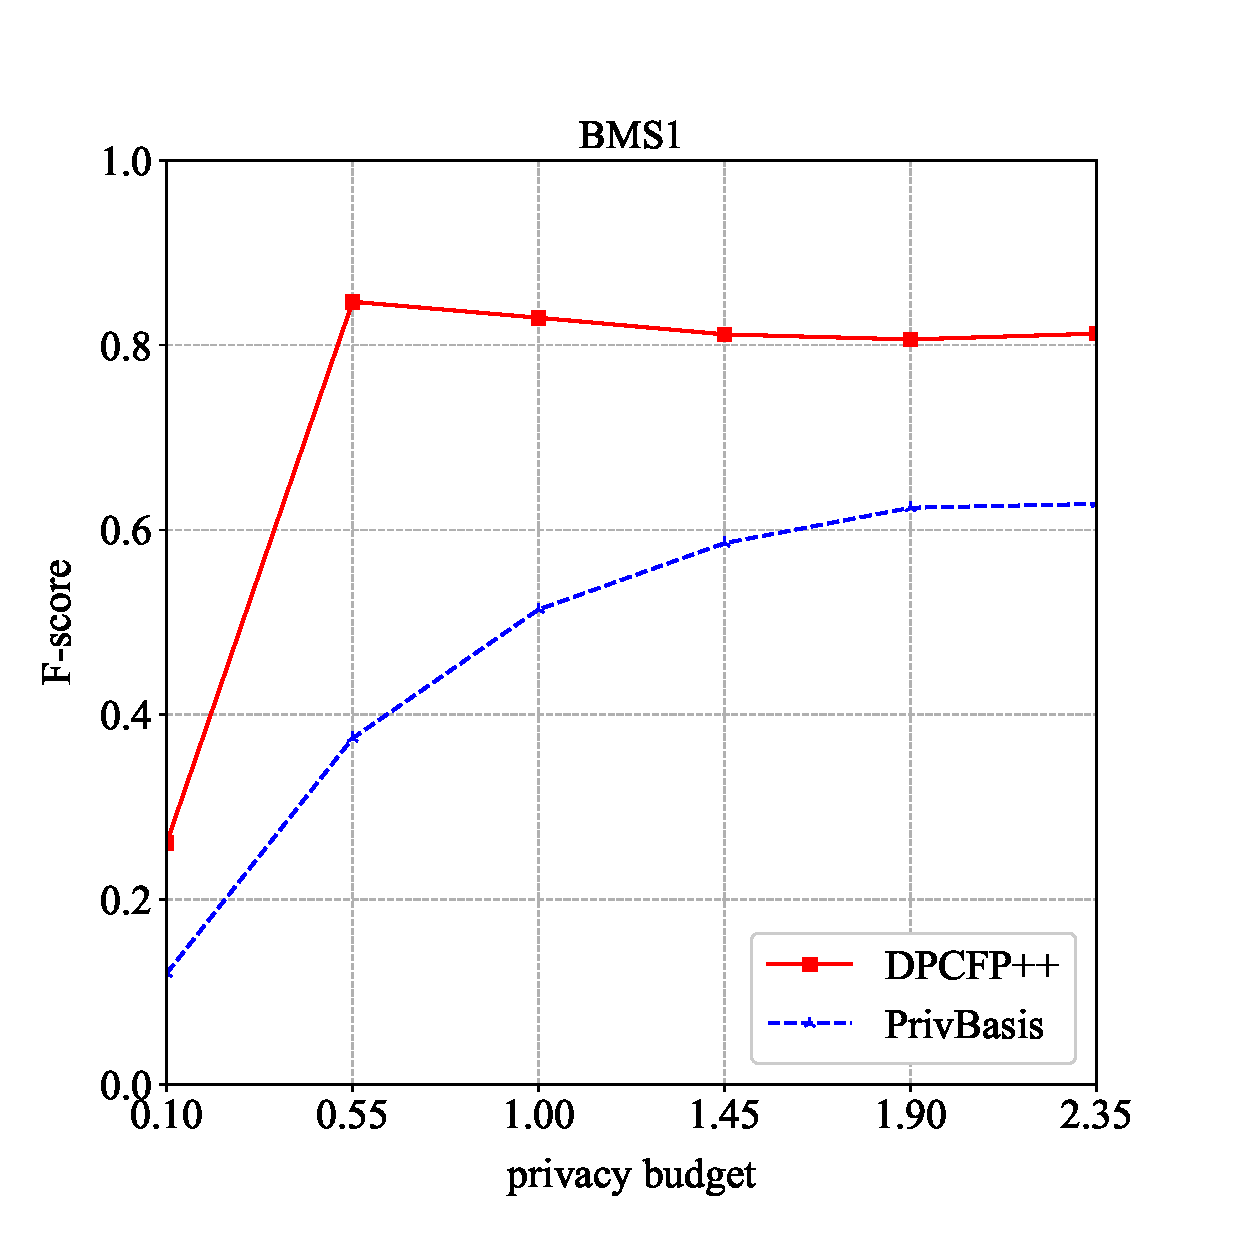
\includegraphics[width=5cm]{F-score_BMS1.eps}
%     \caption{BMS1}
%     \end{minipage}
%     \hfill
%     \begin{minipage}[t]{0.3\textwidth}
%     \centering
%     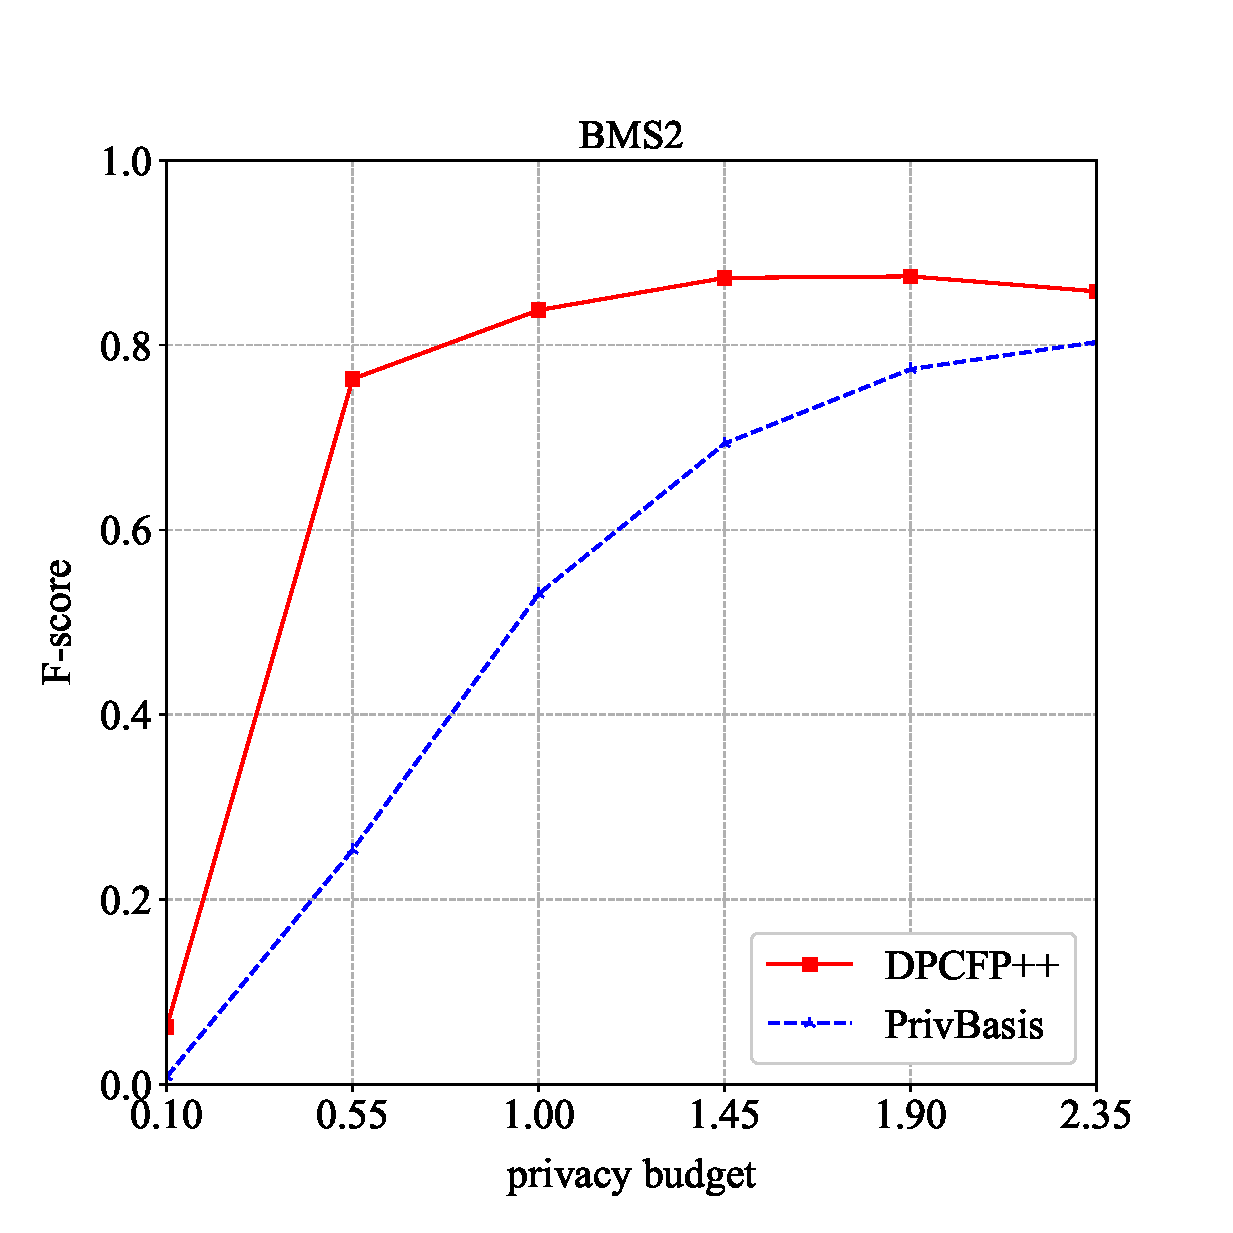
\includegraphics[width=5cm]{F-score_BMS2.eps}
%     \caption{BMS2}
%     \end{minipage}
%     \hfill
%     \begin{minipage}[t]{0.3\textwidth}
%     \centering
%     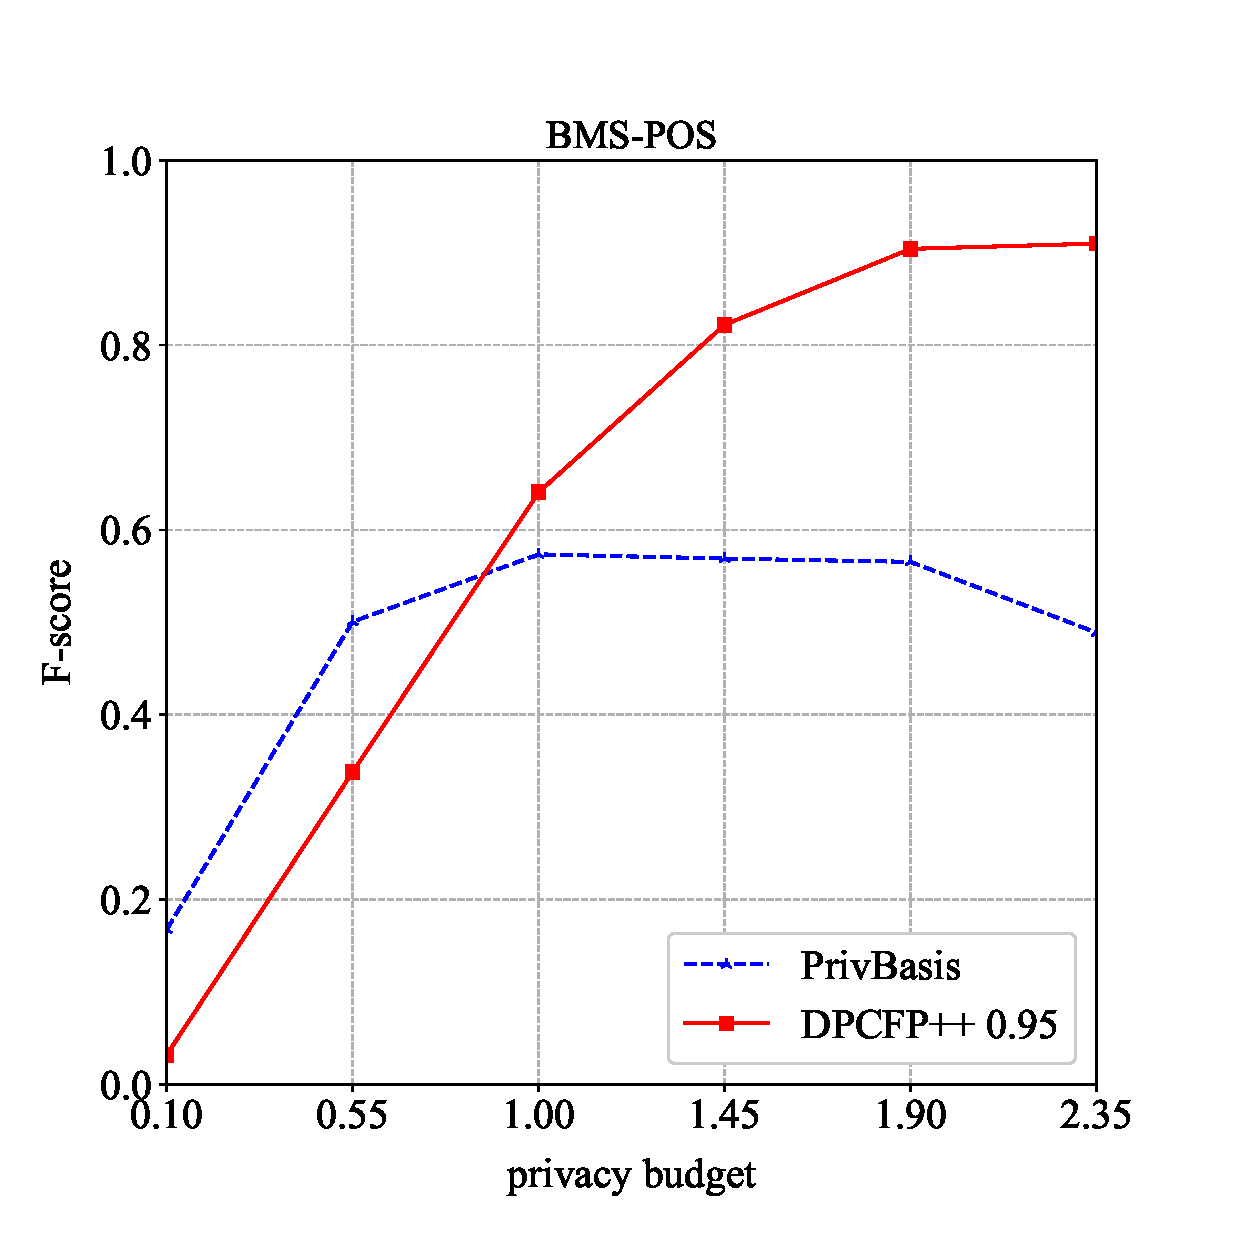
\includegraphics[width=5cm]{F-score_BMS-POS.eps}
%     \caption{BMS-POS}
%     \end{minipage}

%     \begin{minipage}[t]{0.3\textwidth}
%     \centering
%     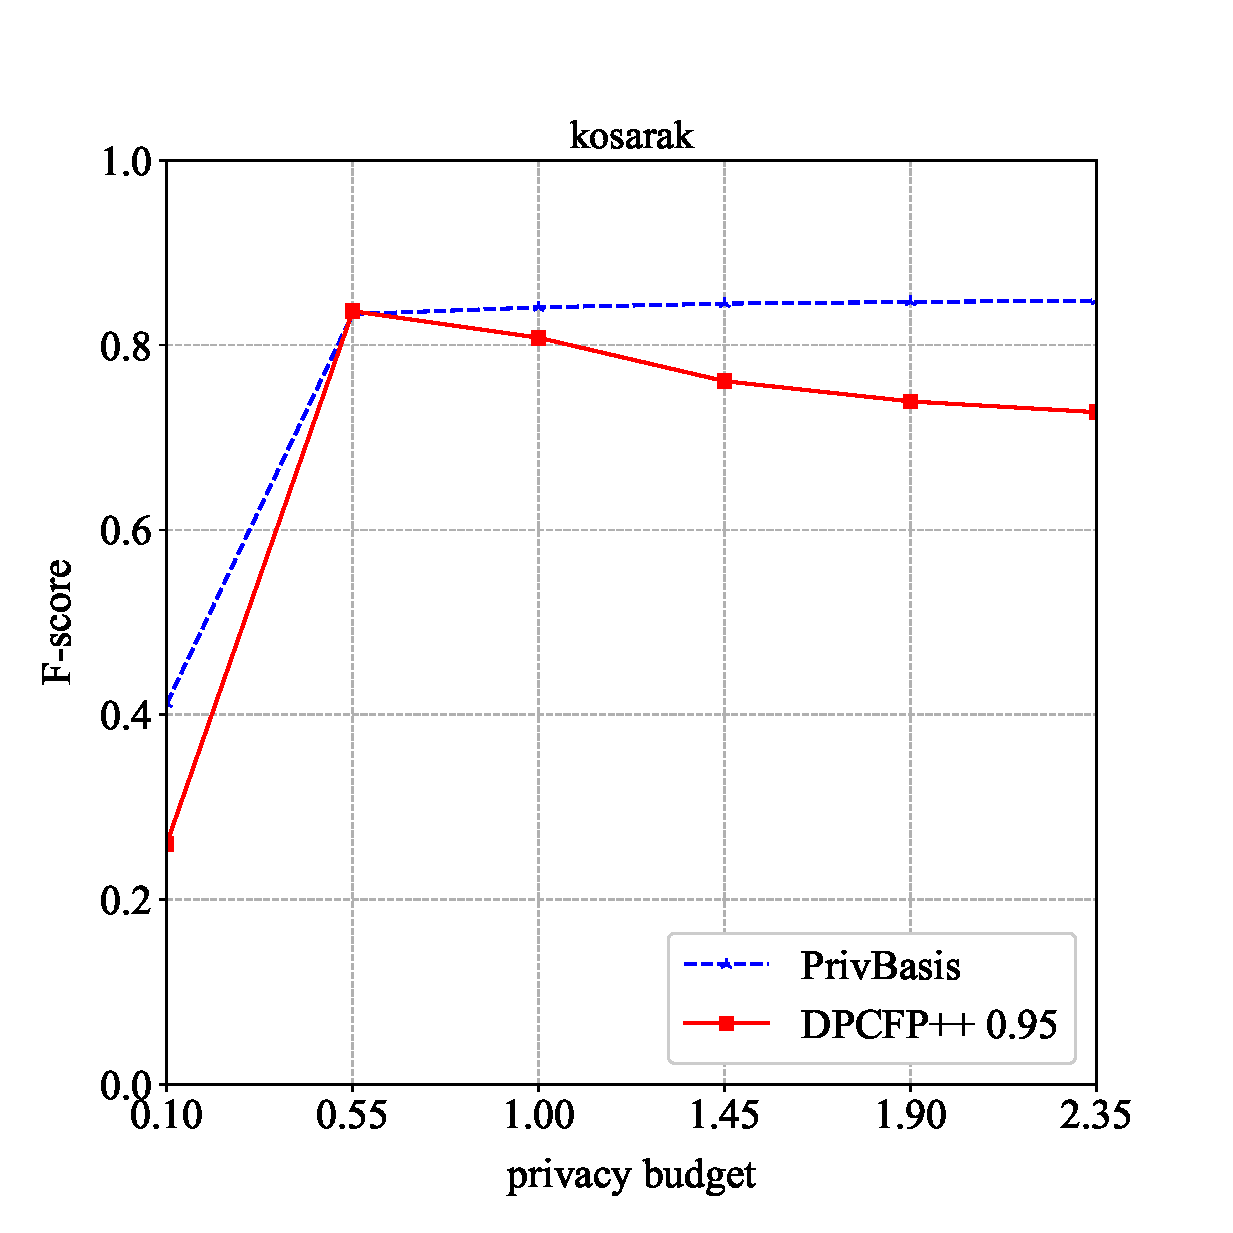
\includegraphics[width=5cm]{F-score_kosarak.eps}
%     % \subcaption{Kosarak}
%     \end{minipage}
%     \hfill
%     \begin{minipage}[t]{0.3\textwidth}
%     \centering
%     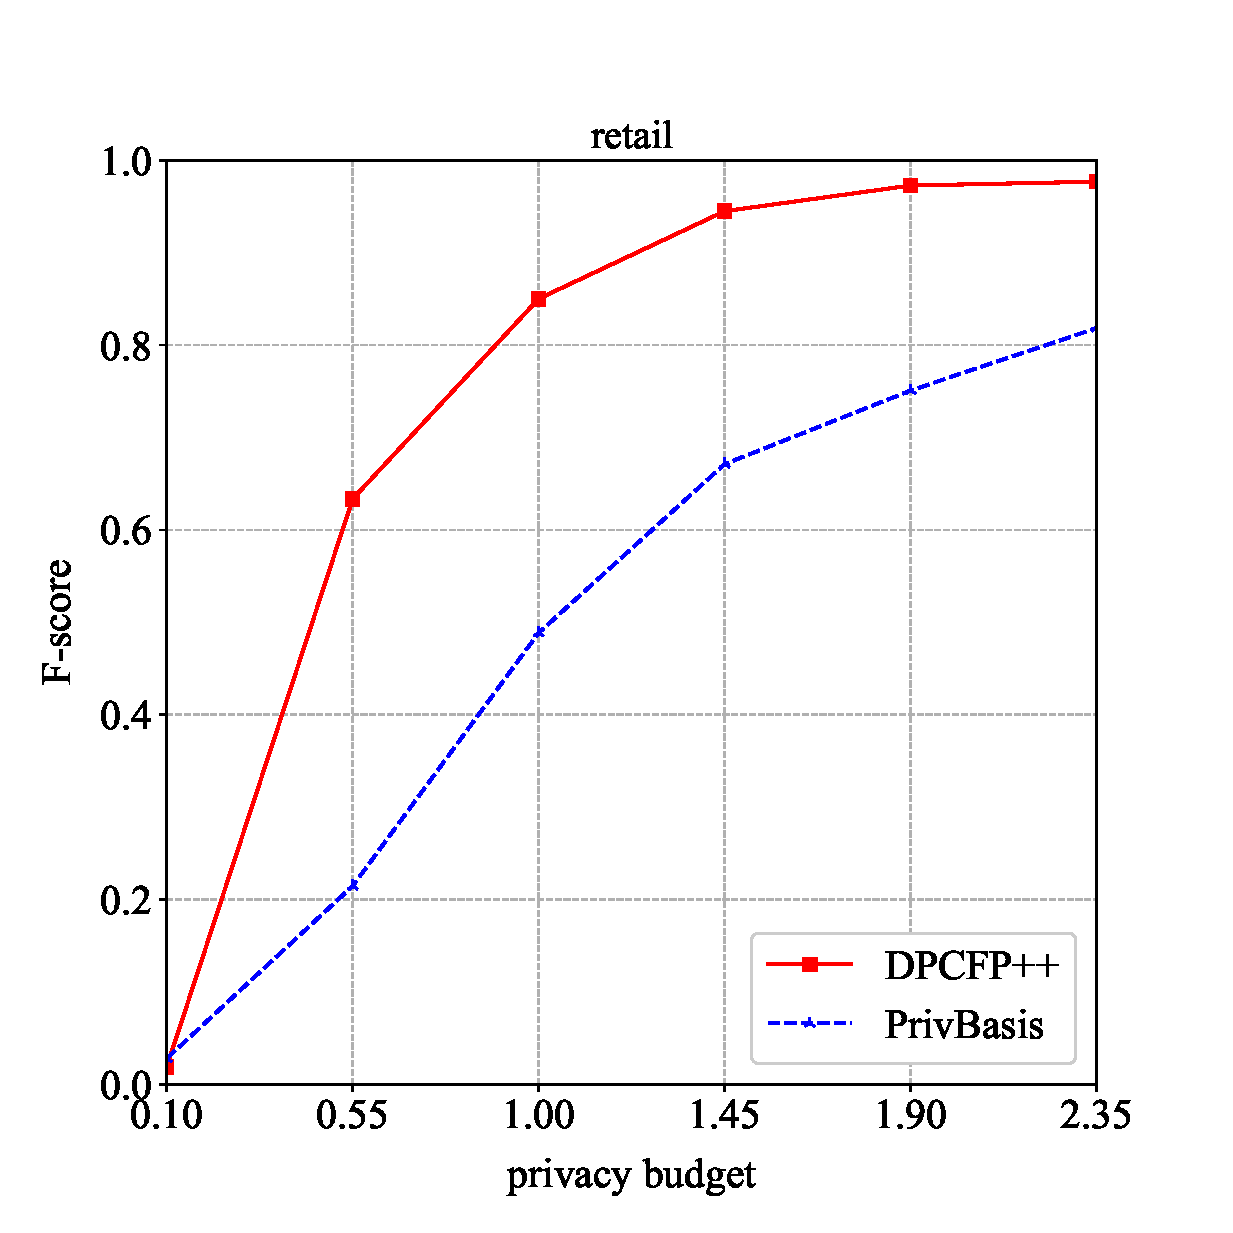
\includegraphics[width=5cm]{F-score_retail.eps}
%     % \subcaption{Retail}
%     \end{minipage}
%     \hfill
%     \begin{minipage}[t]{0.3\textwidth}
%     \centering
%     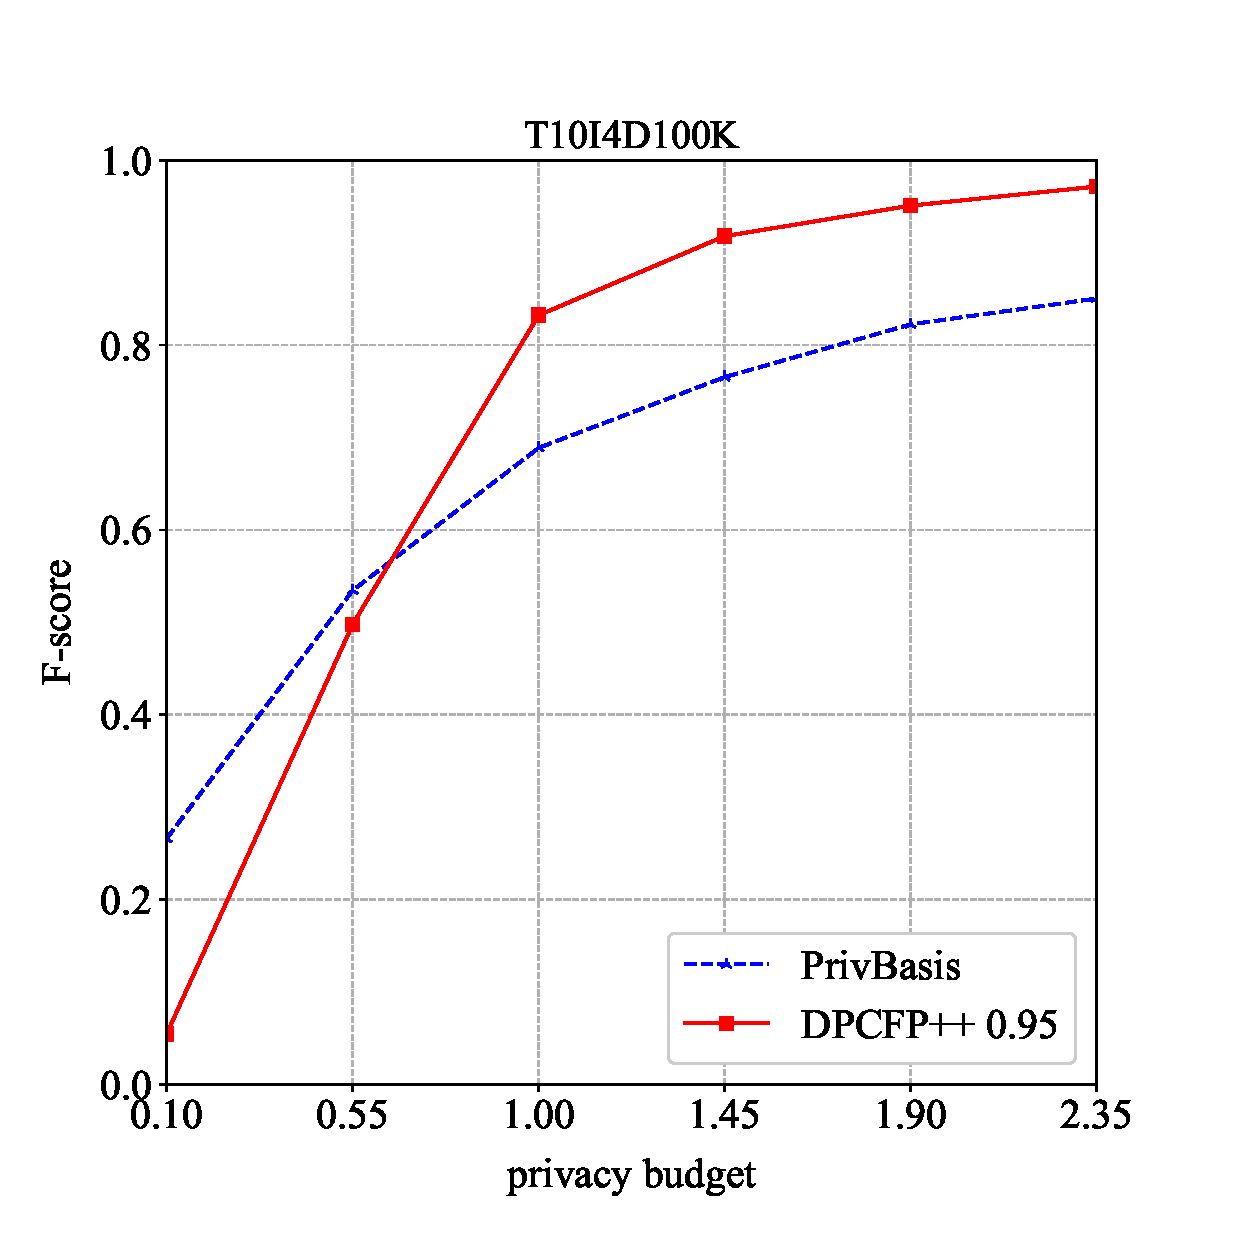
\includegraphics[width=5cm]{F-score_T10I4D100K.eps}
%     % \subcaption{T10I4D100K}
%     \end{minipage}
% \caption{F-score.}
% \label{fig2}
% \end{figure*}

\begin{figure*}[t]
    \centering
    \subfloat[BMS1]{
        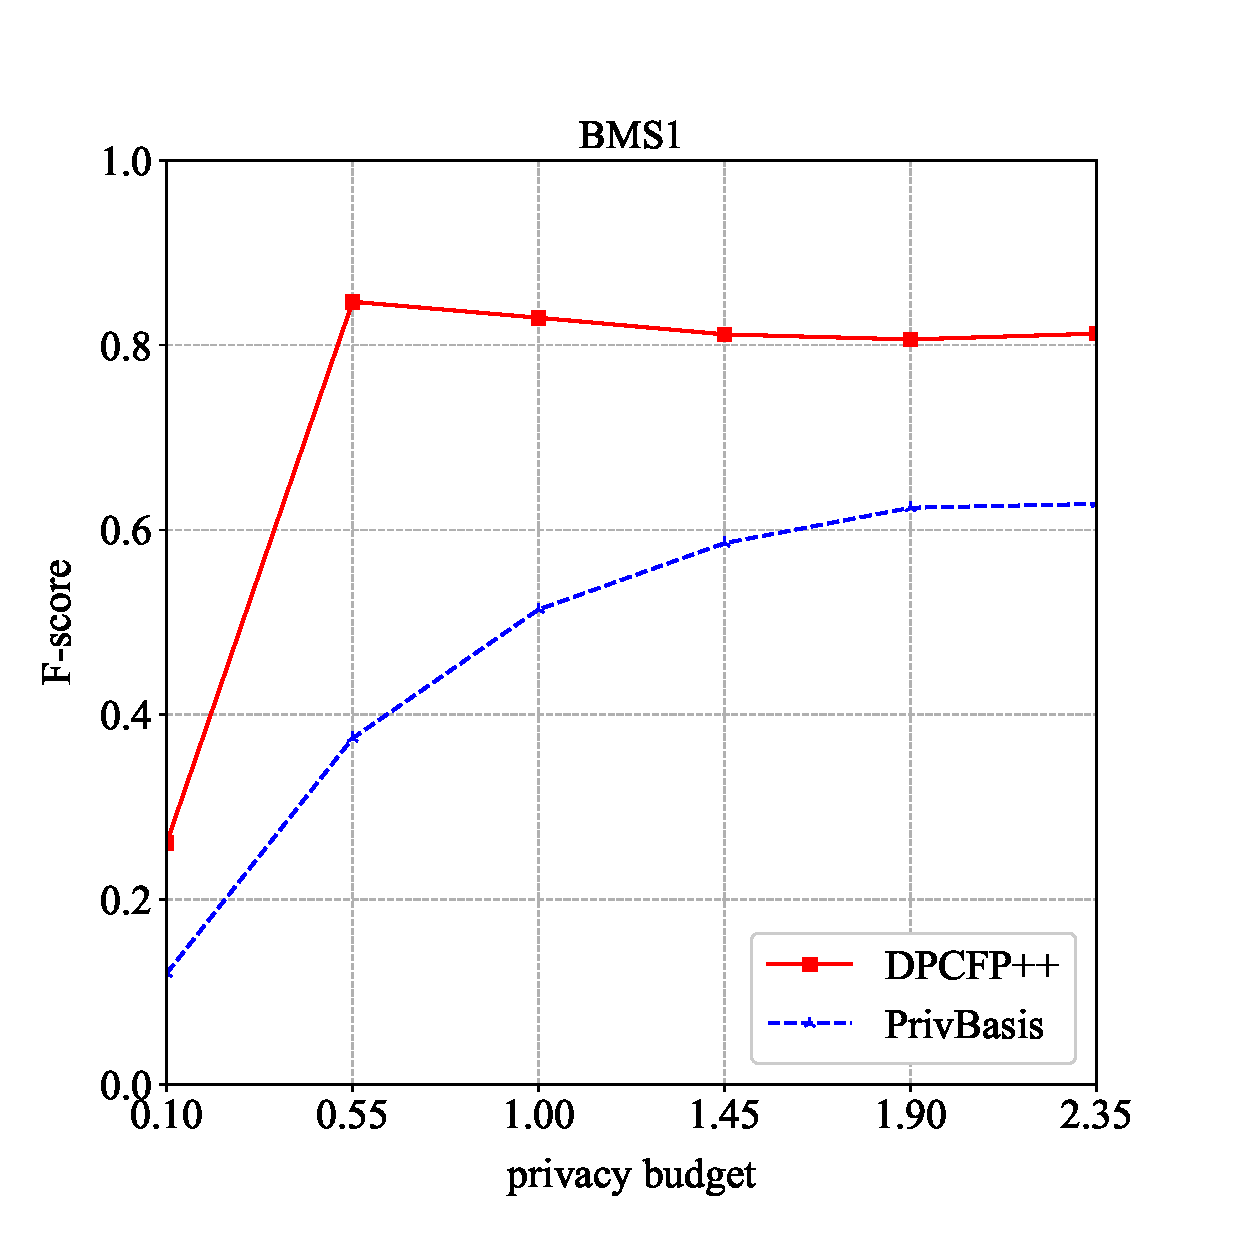
\includegraphics[width=5.5cm]{F-score_BMS1.eps}
    }
    \hfill
    \subfloat[BMS2]{
        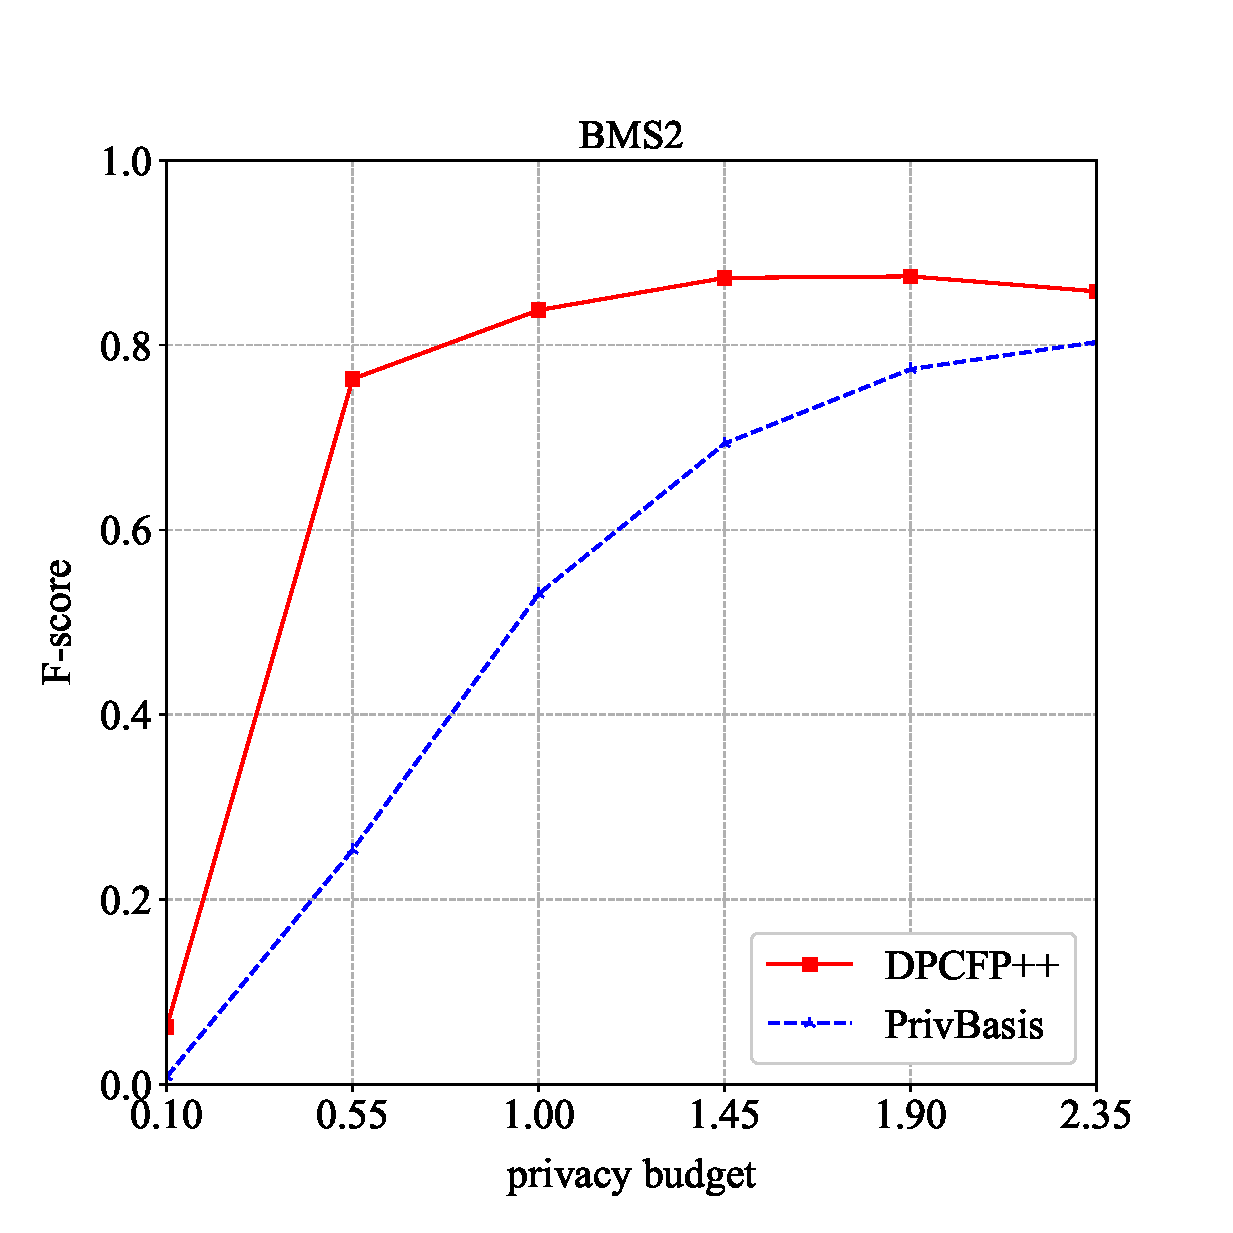
\includegraphics[width=5.5cm]{F-score_BMS2.eps}
    }
    \hfill
    \subfloat[BMS-POS]{
        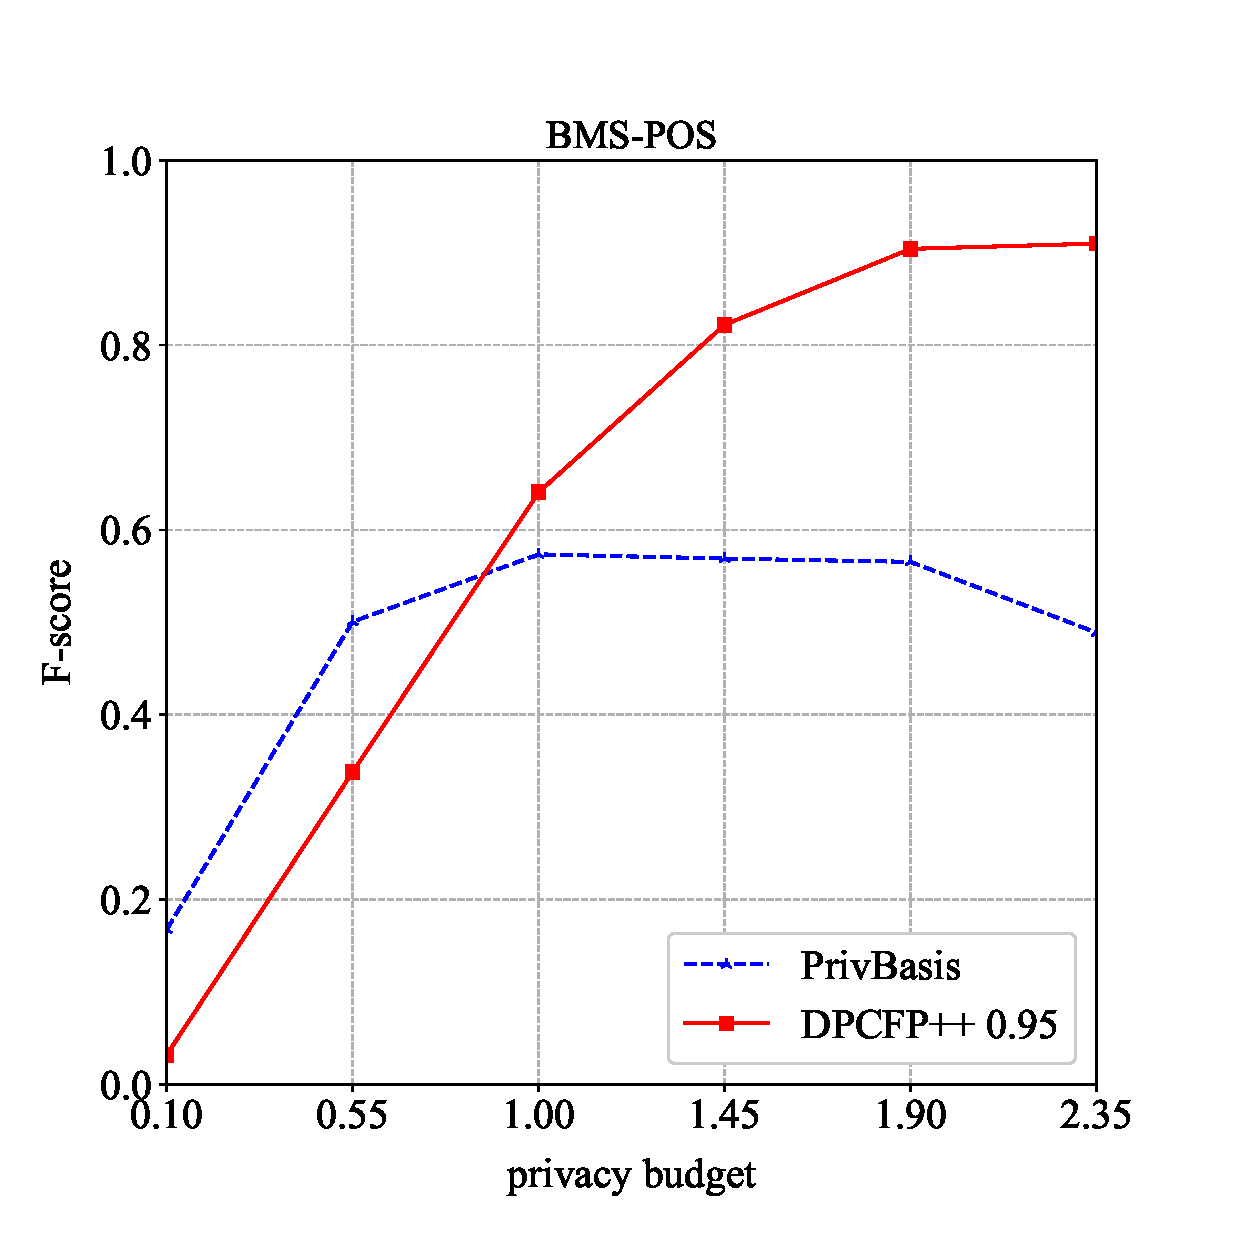
\includegraphics[width=5.5cm]{F-score_BMS-POS.eps}
    }
    \\
    \subfloat[Kosarak]{
        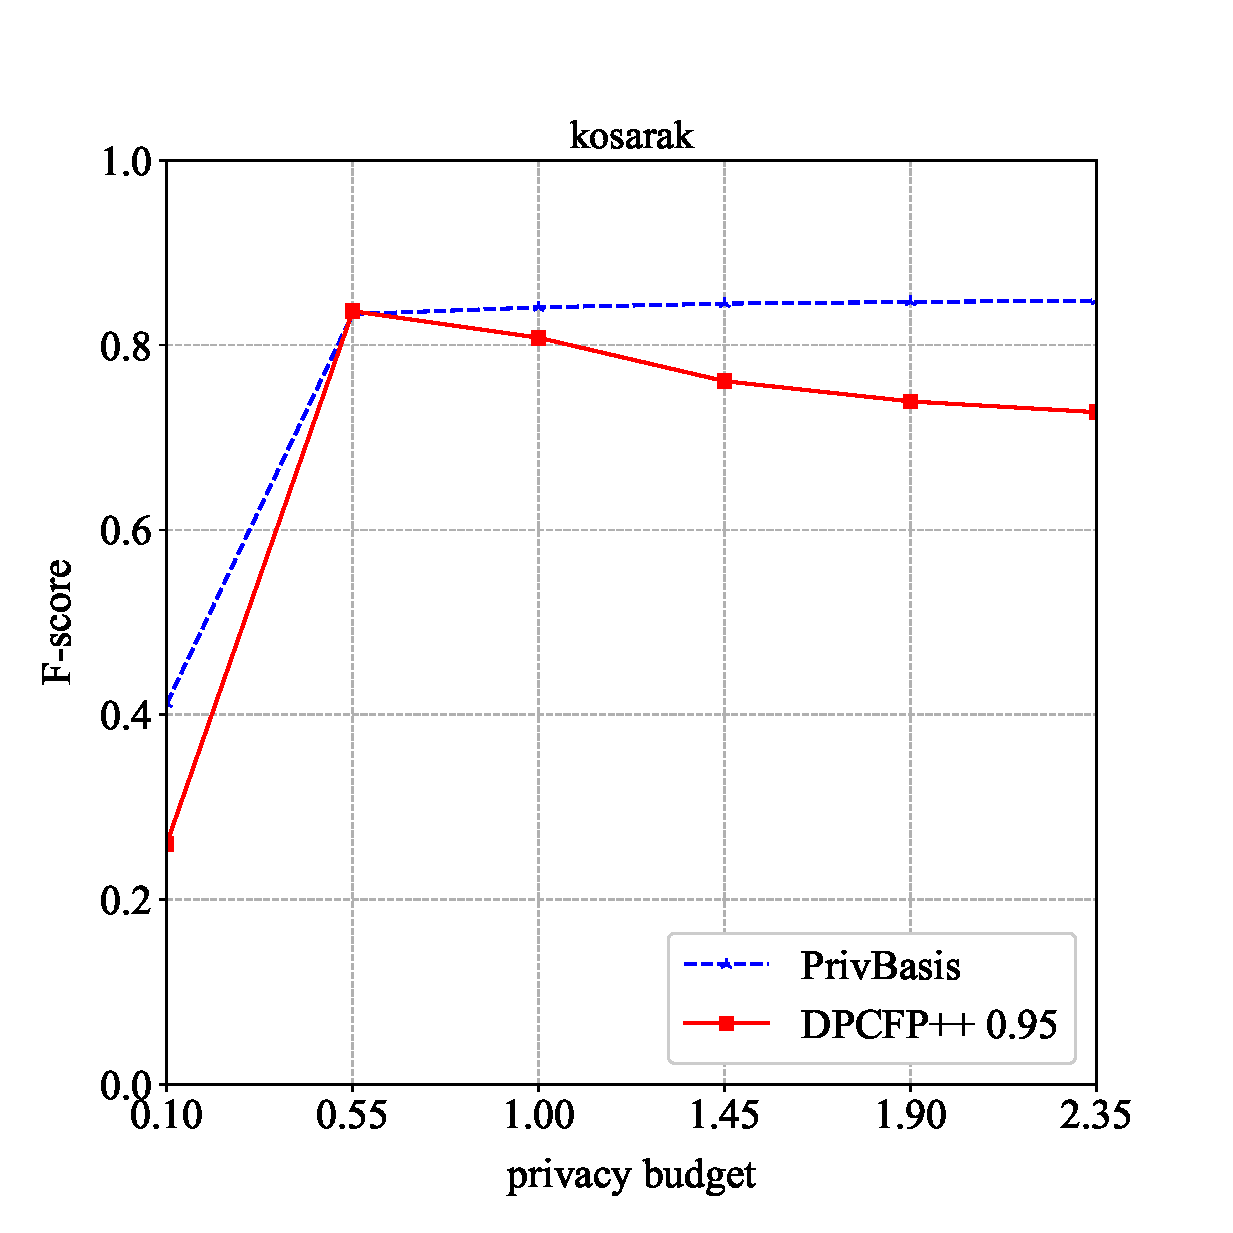
\includegraphics[width=5.5cm]{F-score_kosarak.eps}
    }
    \hfill
    \subfloat[Retail]{
        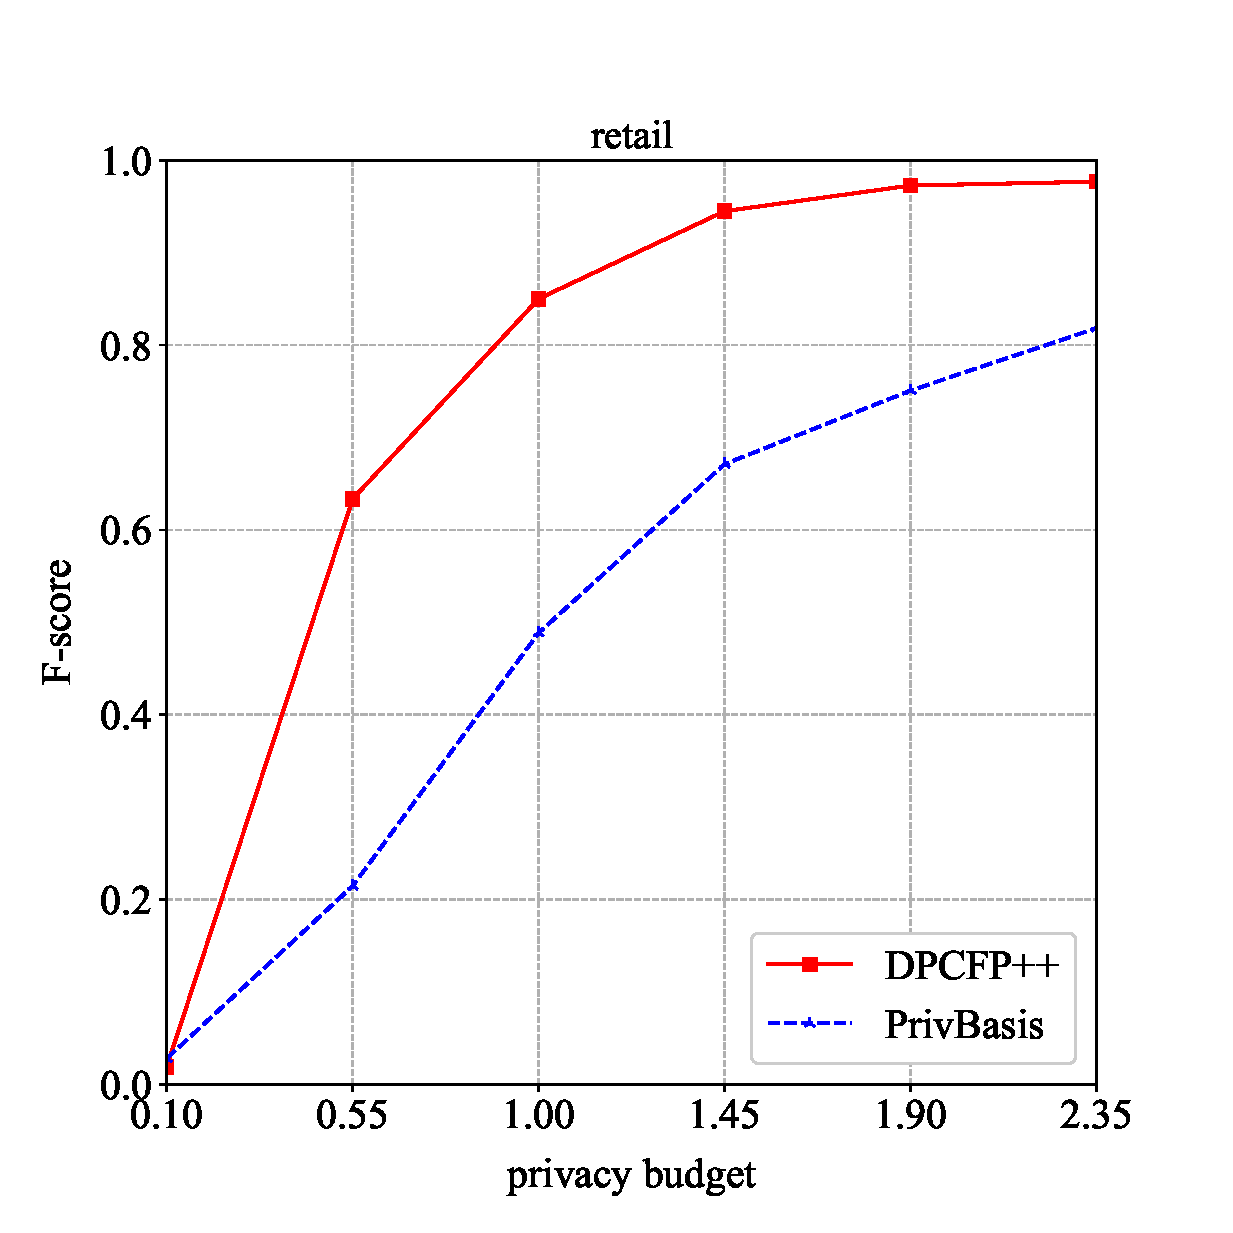
\includegraphics[width=5.5cm]{F-score_retail.eps}
    }
    \hfill
    \subfloat[T10I4D100K]{
        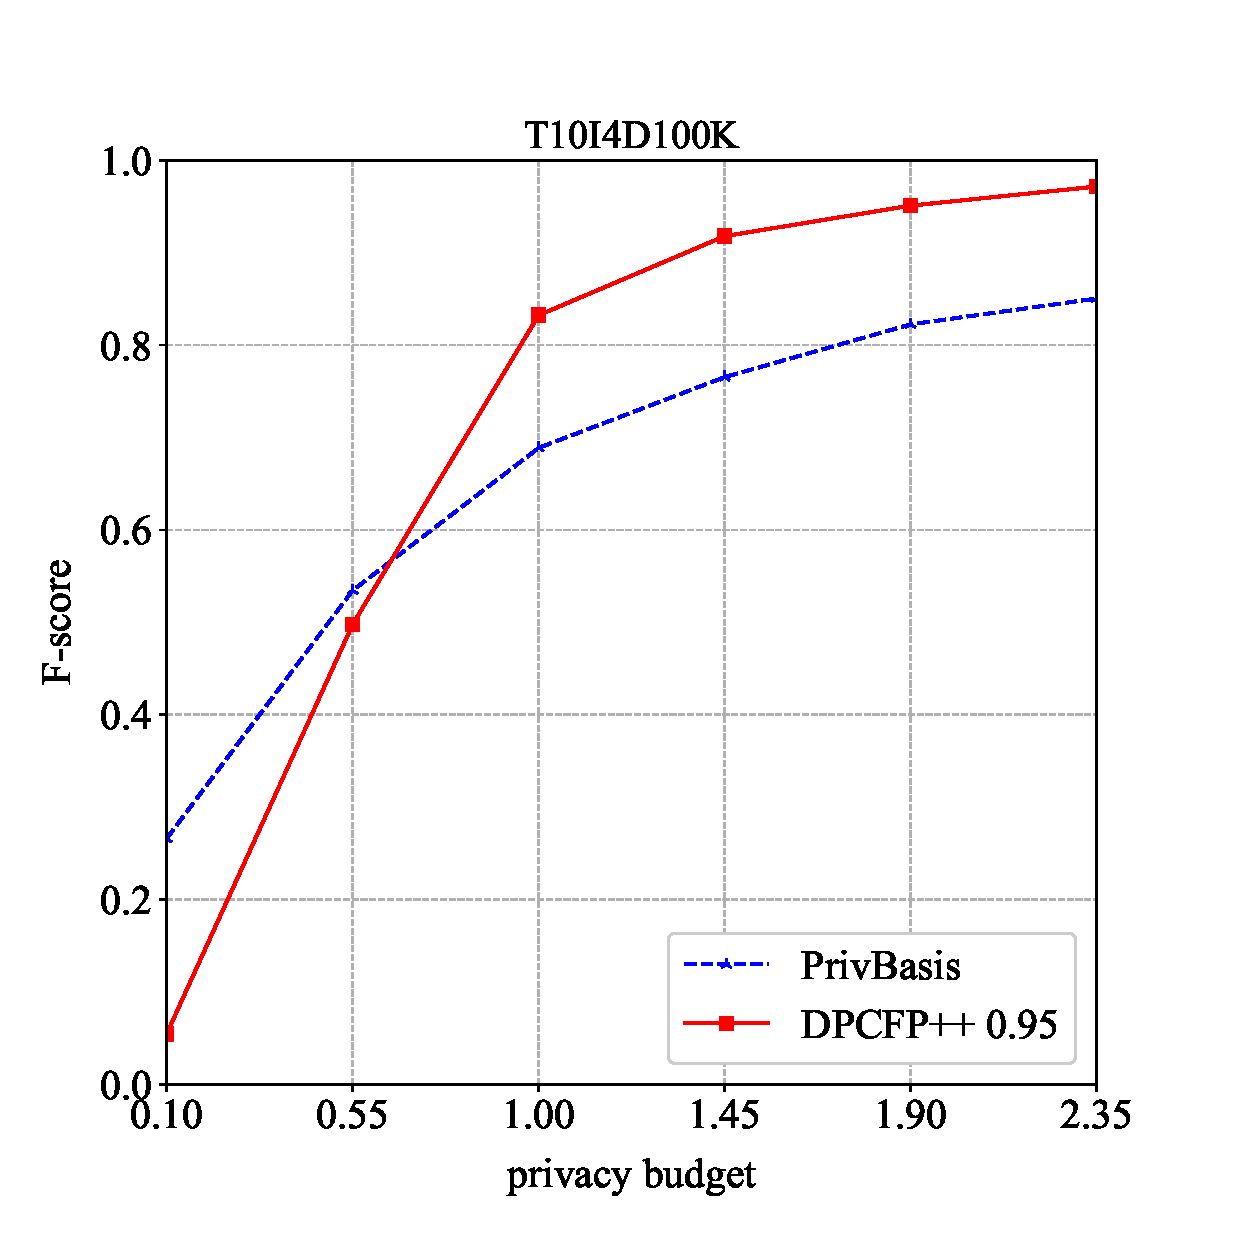
\includegraphics[width=5.5cm]{F-score_T10I4D100K.eps}
    }
\caption{F-score.}
\label{fscore}
\end{figure*}


\begin{figure*}[htbp]
    \centering
    \begin{minipage}[t]{0.3\textwidth}
    \centering
    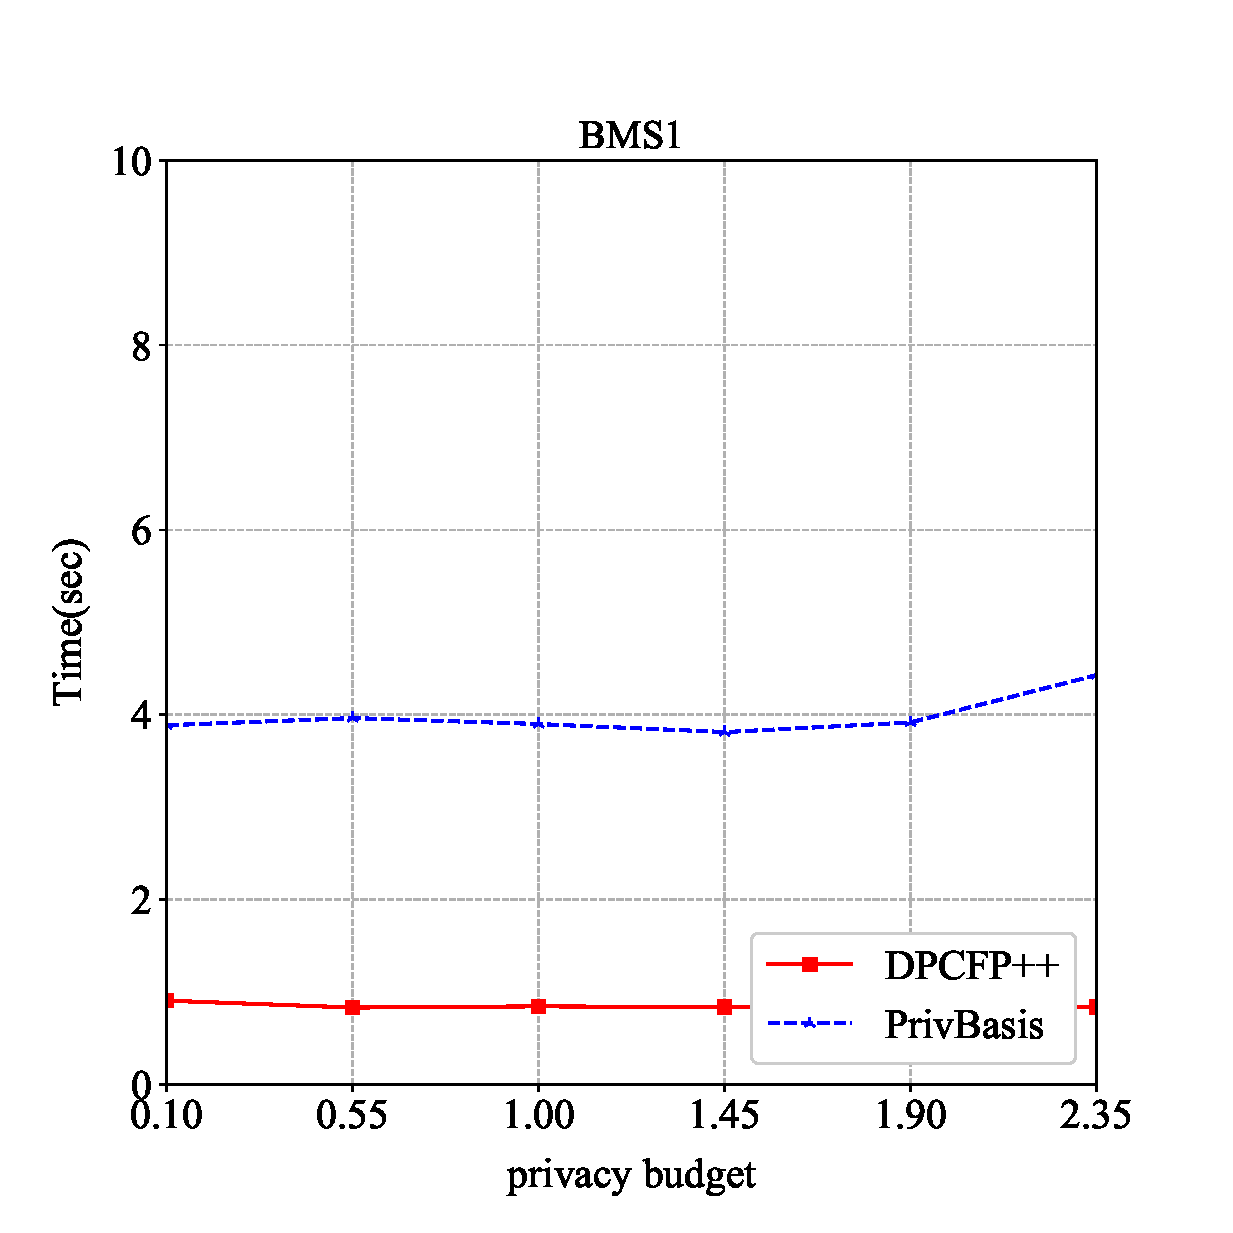
\includegraphics[width=5cm]{Runtime_BMS1.eps}
    % \subcaption{BMS1}
    \end{minipage}
    \hfill
    \begin{minipage}[t]{0.3\textwidth}
    \centering
    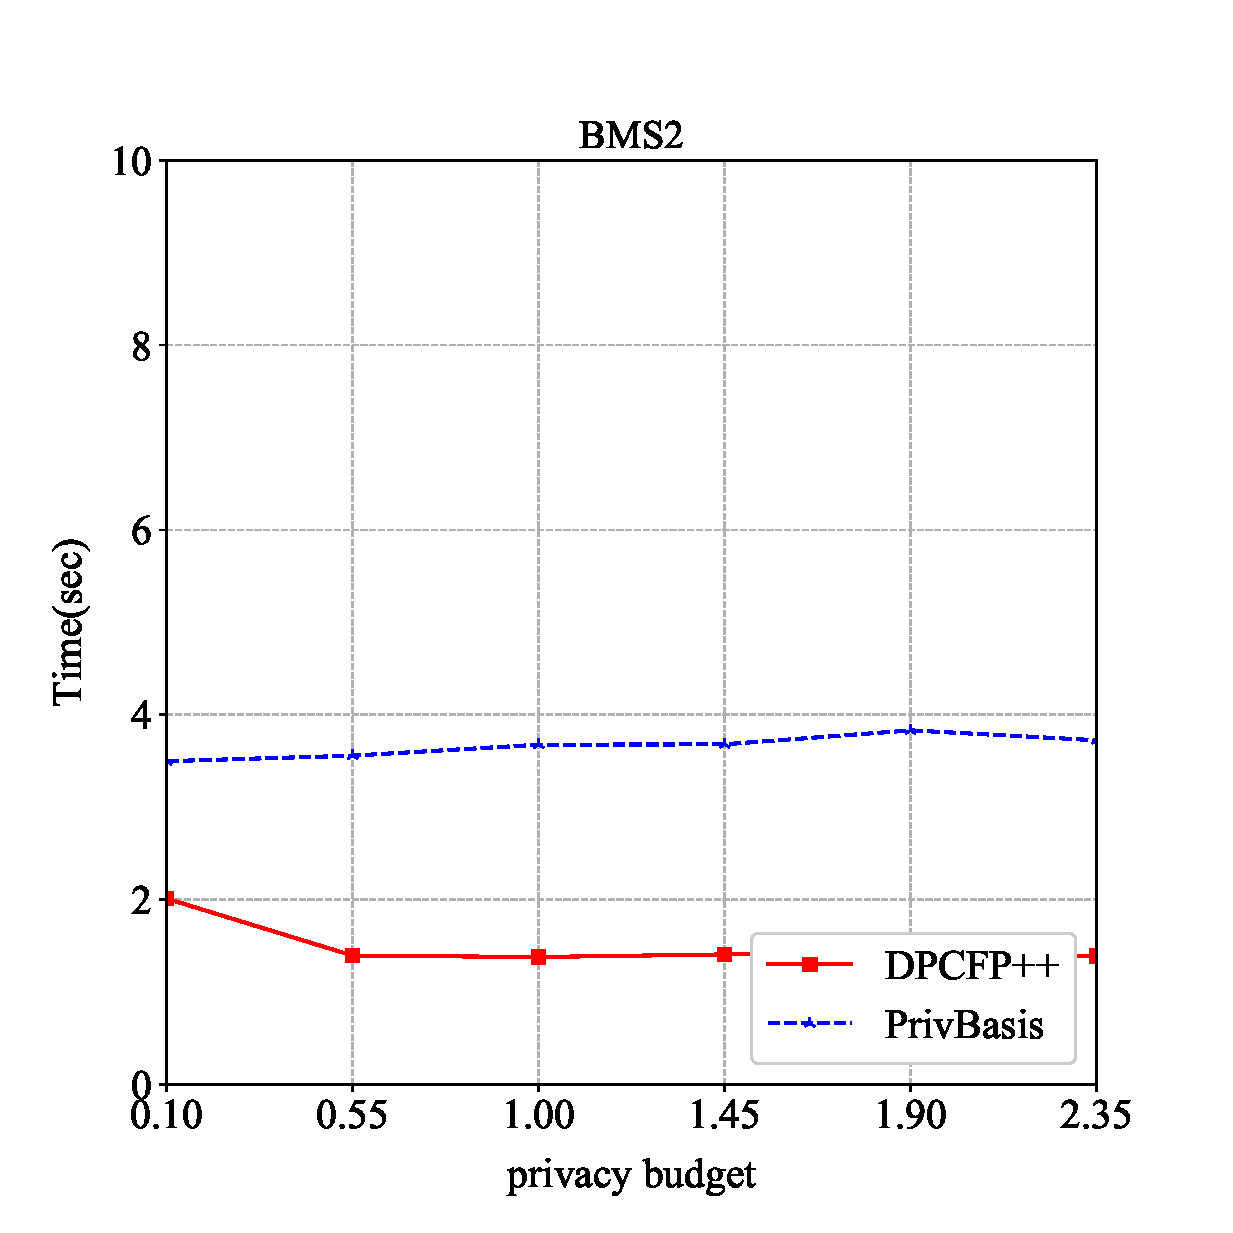
\includegraphics[width=5cm]{Runtime_BMS2.eps}
    % \subcaption{BMS2}
    \end{minipage}
    \hfill
    \begin{minipage}[t]{0.3\textwidth}
    \centering
    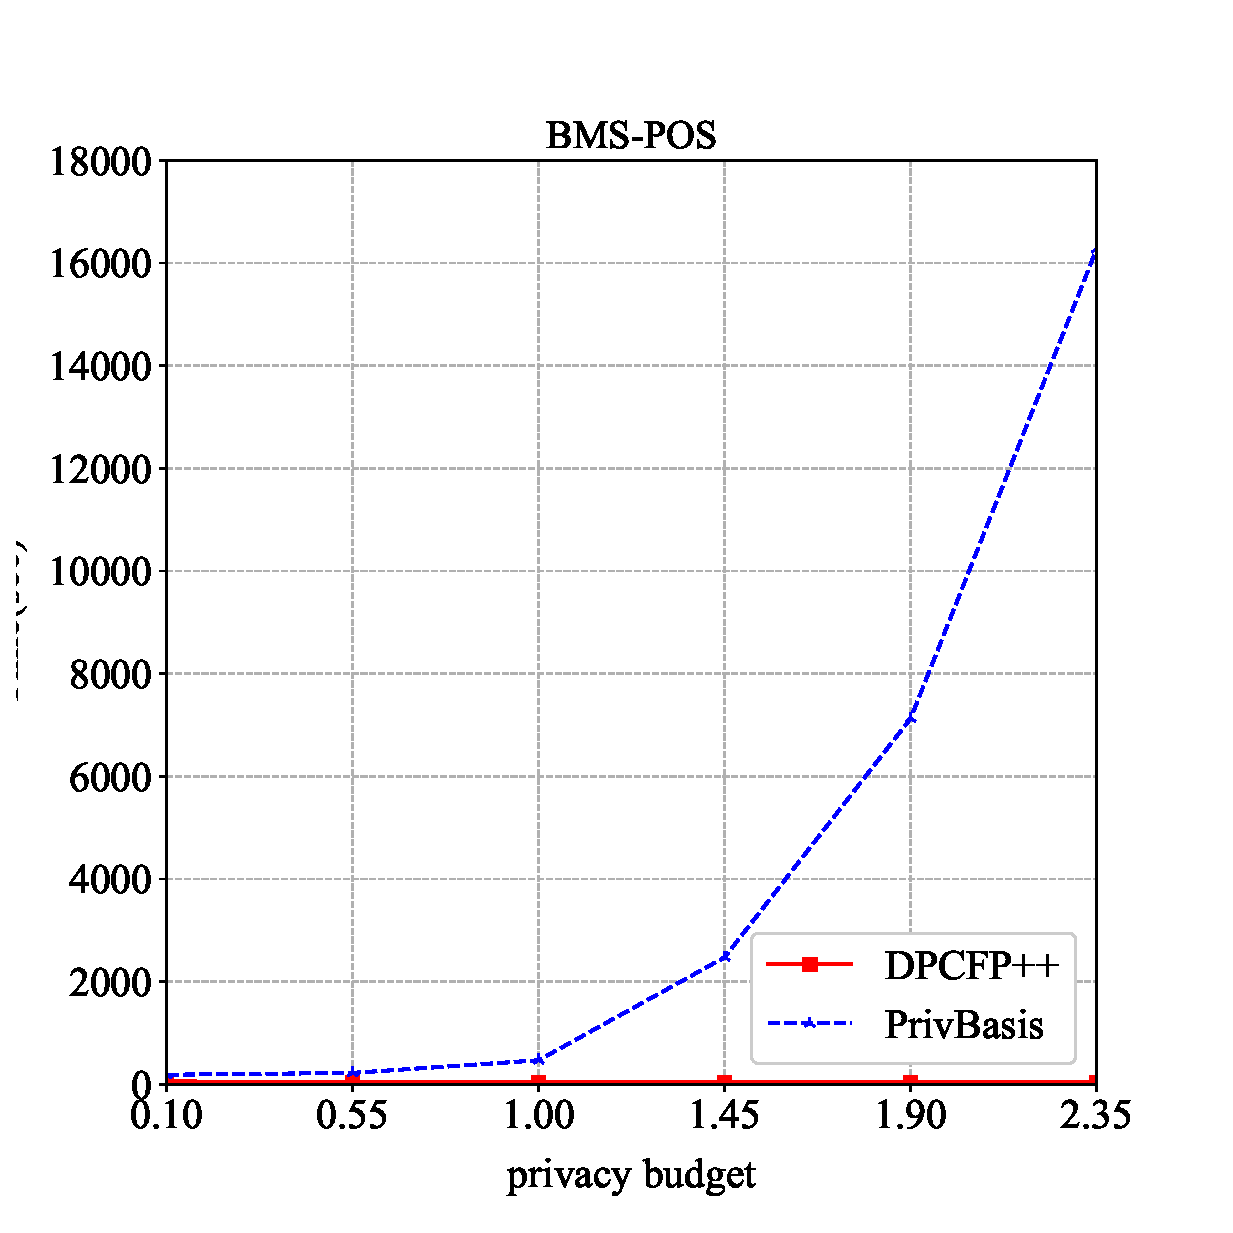
\includegraphics[width=5cm]{Runtime_BMS-POS.eps}
    % \subcaption{BMS-POS}
    \end{minipage}
    
    \begin{minipage}[t]{0.3\textwidth}
    \centering
    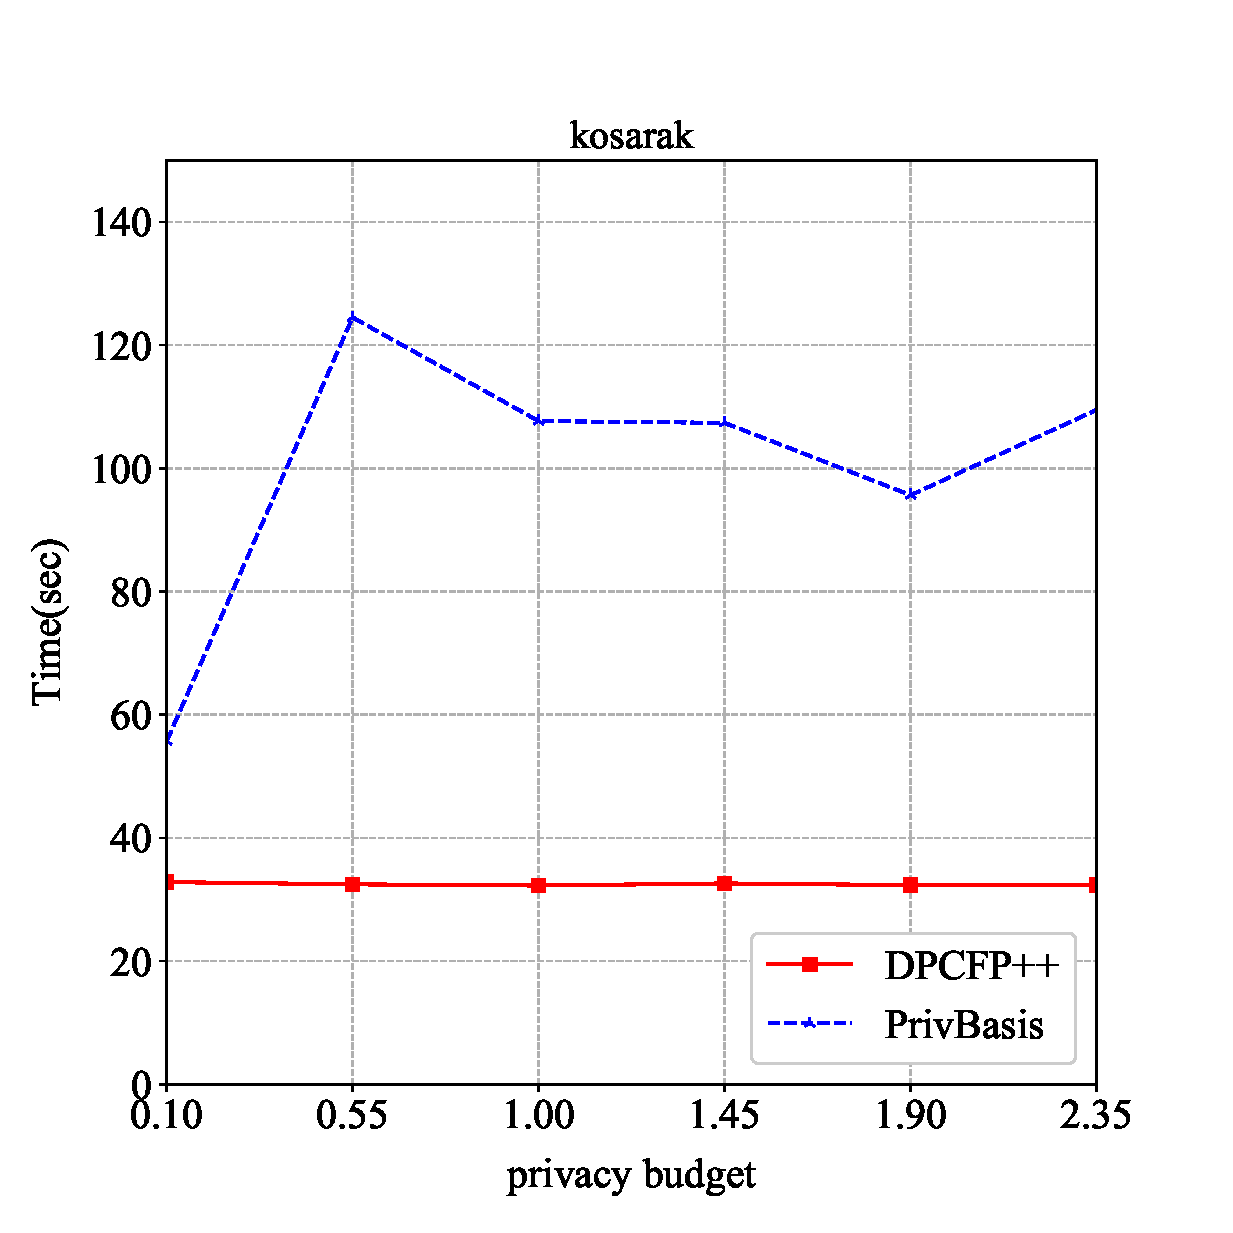
\includegraphics[width=5cm]{Runtime_kosarak.eps}
    % \subcaption{Kosarak}
    \end{minipage}
    \hfill
    \begin{minipage}[t]{0.3\textwidth}
    \centering
    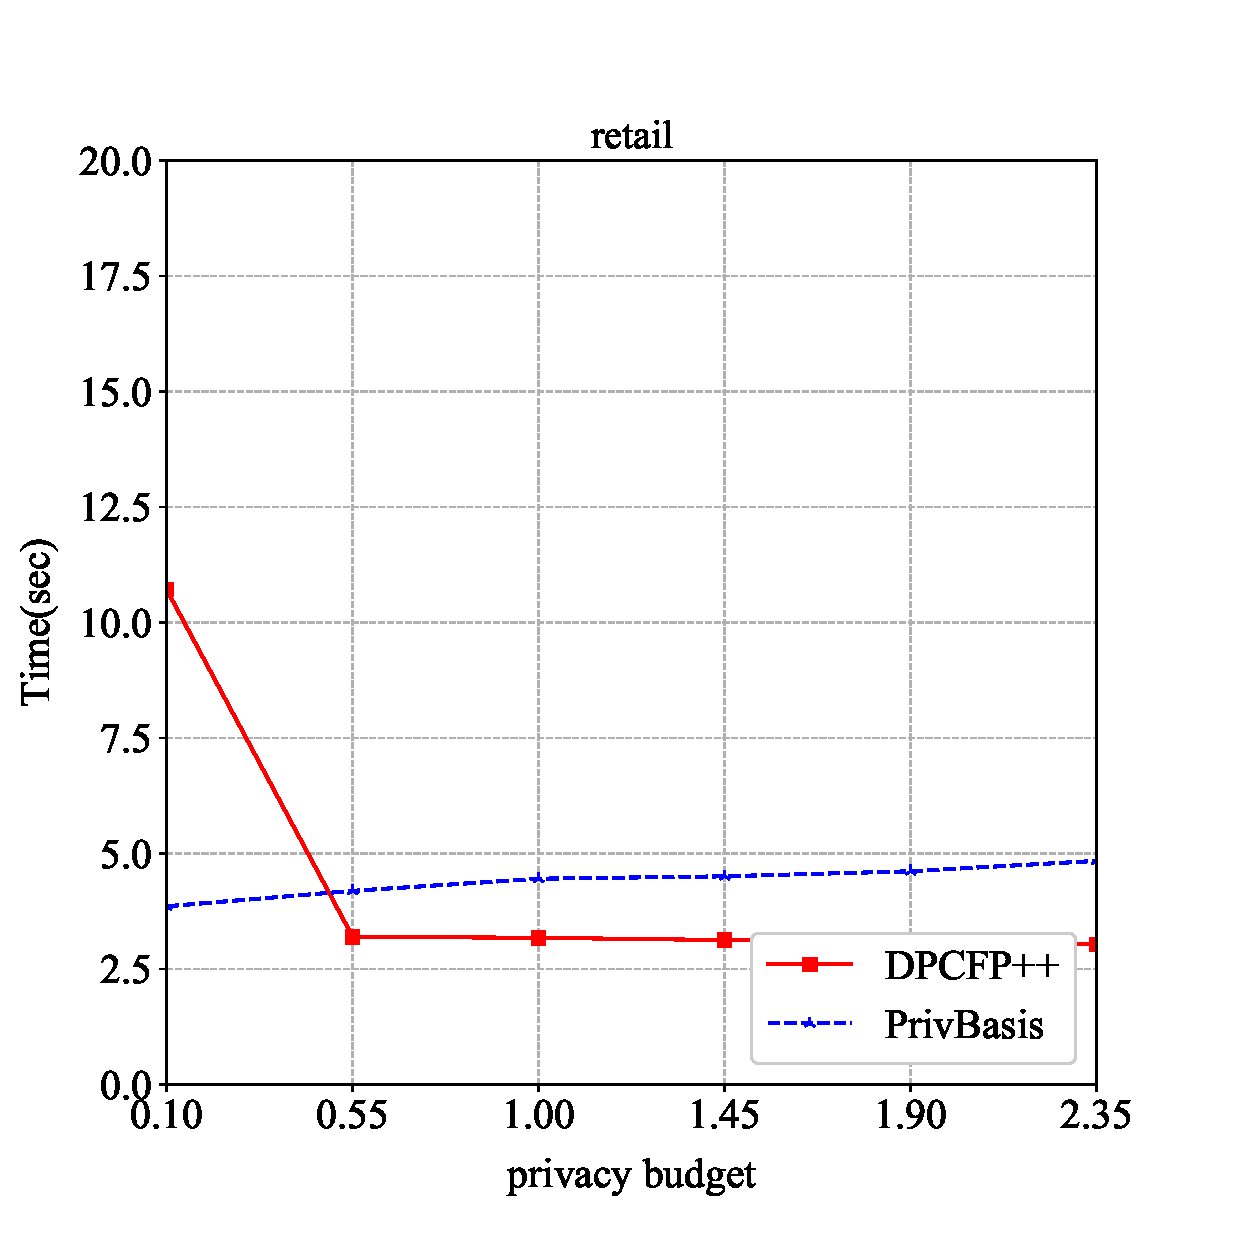
\includegraphics[width=5cm]{Runtime_retail.eps}
    %\subcaption{Retail}
    \end{minipage}
    \hfill
    \begin{minipage}[t]{0.3\textwidth}
    \centering
    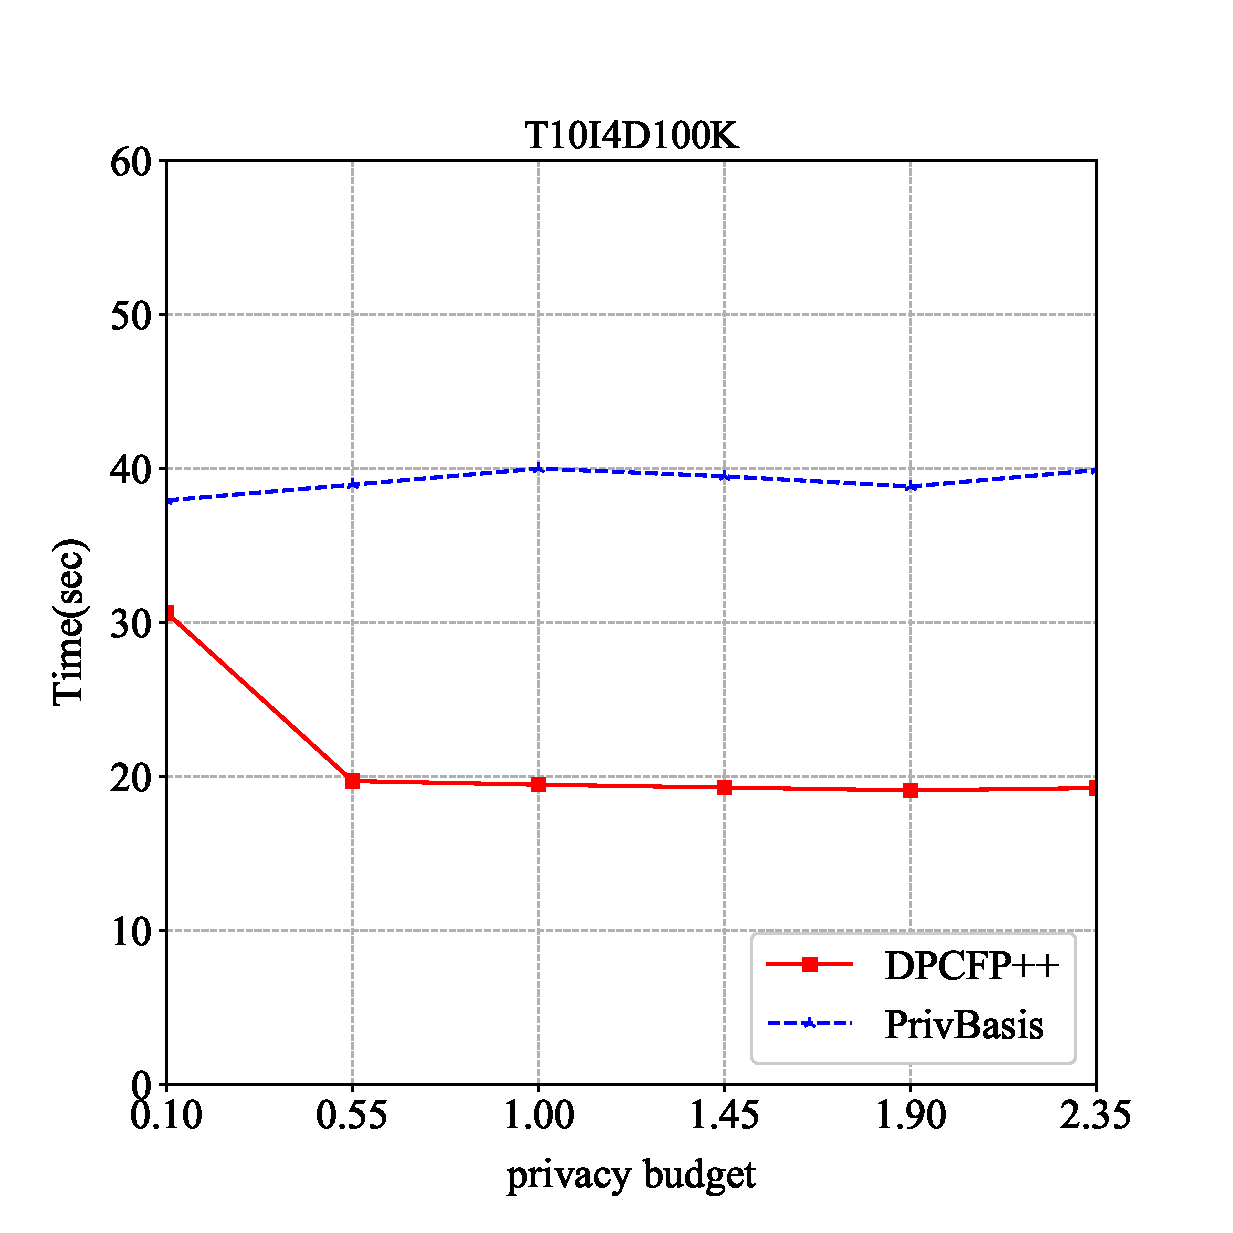
\includegraphics[width=5cm]{Runtime_T10I4D100K.eps}
    %\subcaption{T10I4D100K}
    \end{minipage}
\caption{Runtime.}
\label{fig3}
\end{figure*}

% \section*{References}

% Please number citations consecutively within brackets \cite{b1}. The 
% sentence punctuation follows the bracket \cite{b2}. Refer simply to the reference 
% number, as in \cite{b3}---do not use ``Ref. \cite{b3}'' or ``reference \cite{b3}'' except at 
% the beginning of a sentence: ``Reference \cite{b3} was the first $\ldots$''

% Number footnotes separately in superscripts. Place the actual footnote at 
% the bottom of the column in which it was cited. Do not put footnotes in the 
% abstract or reference list. Use letters for table footnotes.

% Unless there are six authors or more give all authors' names; do not use 
% ``et al.''. Papers that have not been published, even if they have been 
% submitted for publication, should be cited as ``unpublished'' \cite{b4}. Papers 
% that have been accepted for publication should be cited as ``in press'' \cite{b5}. 
% Capitalize only the first word in a paper title, except for proper nouns and 
% element symbols.

\section{Conclusion}
In this paper, we propose a novel differentially private algorithm for frequent itemset mining with multiple minimum supports.


\begin{thebibliography}{00}%論文標題只有第一個字大寫
\bibitem{b1} R. Agrawal, T. Imielinski, and A. Swami. ``Mining association rules between sets of items in large databases,'' in Proceedings of ACM-SIGMOD, 1993.
\bibitem{b2} B. Liu, W. Hsu, and Y. Ma. ``Mining association rules with multiple minimum supports,'' in Proceedings of ACM-SIGKDD, 1999.
\bibitem{b3} Y. Hu, and Y. Chen. ``Mining association rules with multiple minimum supports: a new mining algorithm and a support tuning mechanism,'' in Decision Support System, 2006.
\bibitem{b4} R. Uday Kiran, and P. Krishna Reddy. ``Novel techniques to reduce search space in multiple minimum supports-based frequent pattern mining algorithms,'' in Proceedings of ACM-EDBT, 2011
\bibitem{b5} W. Gan, J. C. Lin, P. Fournier-Viger, H. Chao, and J. Zhan. ``Mining of frequent patterns with multiple minimum supports,'' in Engineering Applications of Artificial Intelligence, 2017
\bibitem{b6} C. Zeng, J. F. Naughton, and J. Cai, ``On differentially private frequent itemset mining,'' in VLDB, 2012.
\bibitem{b7} N. Li, W. H. Qardaji, D. Su, and J. Cao, ``Privbasis: frequent itemset mining with differential privacy,'' in PVLDB, 2012.
\bibitem{b8} J. Lee and C. W. Clifton, ``Top-k frequent itemsets via differentially private fp-trees,'' in KDD, 2014.
\bibitem{b9} C. Dwork. Differential privacy. In ICALP, 2006.
\bibitem{b10}Y. Chen and A. Machanavajjhala, “On the privacy properties of variants on the sparse vector technique,” CoRR, 2015.
\bibitem{b11}J. Zhang, X. Xiao, and X. Xie, “Privtree: A differentially private algorithm for hierarchical decompositions,” in SIGMOD, 2016.

\end{thebibliography}


\end{document}
